 
% example for dissertation.sty
\documentclass[
  % Replace oneside by twoside if you are printing your thesis on both sides
  % of the paper, leave as is for single sided prints or for viewing on screen.
  oneside,
  %twoside,
  11pt, a4paper,
  footinclude=true,
  headinclude=true,
  cleardoublepage=empty
]{scrbook}

\usepackage{dissertation}
\usepackage[utf8]{inputenc} %Needed for PT letters unavailable to EN language ( ç,....)
\usepackage{amsmath,mathtools,calc}
\usepackage{footnote}
\usepackage{hyperref}
\usepackage{multirow}
\usepackage[normalem]{ulem}


\usepackage{listings}
%LISTING - GENERAL
\lstset{
	basicstyle=\small,
	keywords={},
	numbers=left,
	numberstyle=\tiny,
	numbersep=5pt,
	breaklines=true,
	stepnumber=1,
    	frame=tB,
	%mathescape=true,
	escapeinside={(*@}{@*)}
}
%
%\lstset{ %
%	language=Java,							% choose the language of the code
%	basicstyle=\ttfamily\footnotesize,		% the size of the fonts that are used for the code
%	keywordstyle=\bfseries,					% set the keyword style
%	%numbers=left,							% where to put the line-numbers
%	numberstyle=\scriptsize,				% the size of the fonts that are used for the line-numbers
%	stepnumber=2,							% the step between two line-numbers. If it's 1 each line
%											% will be numbered
%	numbersep=5pt,							% how far the line-numbers are from the code
%	backgroundcolor=\color{white},			% choose the background color. You must add \usepackage{color}
%	showspaces=false,						% show spaces adding particular underscores
%	showstringspaces=false,					% underline spaces within strings
%	showtabs=false,							% show tabs within strings adding particular underscores
%	frame=none,								% adds a frame around the code
%	%abovecaptionskip=-.8em,
%	%belowcaptionskip=.7em,
%	tabsize=2,								% sets default tabsize to 2 spaces
%	captionpos=b,							% sets the caption-position to bottom
%	breaklines=true,						% sets automatic line breaking
%	breakatwhitespace=false,				% sets if automatic breaks should only happen at whitespace
%	title=\lstname,							% show the filename of files included with \lstinputlisting;
%											% also try caption instead of title
%	escapeinside={\%*}{*)},					% if you want to add a comment within your code
%	morekeywords={*,...}					% if you want to add more keywords to the set
%}

% ACRONYMS -----------------------------------------------------

%import the necessary package with some options
\usepackage[acronym,nonumberlist,nomain]{glossaries}

%enable the following to avoid links from the acronym usage to the list
%\glsdisablehyper

%displays the first use of an acronym in italic
\defglsdisplayfirst[\acronymtype]{\emph{#1#4}}


%the style of the Glossary
\glossarystyle{listgroup}

% set the name for the acronym entries page
\renewcommand{\glossaryname}{Acronyms}

%this shall be the last thing in the acronym configuration!!
\makeglossaries


% here are the acronym entries
\newacronym{mei}{MEI}{Mestrado em Engenharia Informática}
\newacronym{di}{DI}{Departamento de Informática}
\newacronym{um}{UM}{Universidade do Minho}

\newacronym{qos}{QoS}{Quality of Service}
\newacronym{soa}{SOA}{Service Oriented Architecture}

% these could go in an acronyms.tex file, and loaded with:
% \loadglsentries[\acronymtype]{Parts/Definitions/acronyms}
% when using this, you may want to remove 'nomain' from the package options

%% **MORE INFO** %%

%to add the acronyms list add the following where you want to print it:
%\printglossary[type=\acronymtype]
%\clearpage
%\thispagestyle{empty}

%to use an acronym:
%\gls{qps}

% compile the thesis in command line with the following command sequence:
% pdlatex dissertation.tex
% makeglossaries dissertation
% bibtex dissertation
% pdlatex dissertation.tex
% pdlatex dissertation.tex

% ----------------------------------------------------------------

% Title
\titleA{Implementing a Syntax Directed Editor}
\titleB{for LISS.} % (if any)
%\titleB{for LogoLISS with incremental compilation} % (if any)
%\subtitleA{First Part of Subtitle}
%\subtitleB{Second part of Subtitle} % (if any)

% Author
\author{Damien da Silva Vaz}

% Supervisor(s)
\supervisor{Professor Pedro Rangel Henriques}
\cosupervisor{Professor Daniela da Cruz}

% University (uncomment if you need to change default values)
% \def\school{Escola de Engenharia}
% \def\department{Departamento de Inform\'{a}tica}
% \def\university{Universidade do Minho}
% \def\masterdegree{Computer Science}

% Date
\date{\myear} % change to text if date is not today

% Keywords
%\keywords{master thesis}

% Glossaries & Acronyms
%\makeglossaries  %  either use this ...
%\makeindex	   % ... or this

% Define Acronyms
%%!TEX root = ../dissertation.tex

\newacronym{mei}{MEI}{Mestrado em Engenharia Inform\'{a}tica}
\newacronym{um}{UM}{Universidade do Minho}
%\glsaddall[types={\acronymtype}]



\ummetadata % add metadata to the document (author, publisher, ...)

\begin{document}
	% Cover page ---------------------------------------
	\umfrontcover	
	\umtitlepage
	
	% Add acknowledgements ----------------------------
	\chapter*{Acknowledgements}
	Firstly, I would like to thank my supervisor Pedro Rangel Henriques and co-supervisor Daniela da Cruz. They are the most who supported me throw this ambitious project and took me to the final stage of my university career.\newline
Thank you also to my family and friends (Ranim, Bruno, Chloé, Tiago, Tamara, Saozita, Nuno, David, Natália) for supporting me.\newline
And last but not least, I would like to dedicate this thesis to my, particularly, most beautiful mother.
Despite you couldn't be here to watch me conclude my studies. Wherever you are, I hope that you are proud of me.	
None of this could have been made without their unconditional help.

	% Add abstracts (en,pt) ---------------------------
	\chapter*{Abstract}
	The aim of this master work is to implement LISS language in ANTLR compiler generator system using an attribute grammar which create an abstract syntax tree (AST) and generate MIPS assembly code for MARS (MIPS Assembler and Runtime Simulator) .
Using that AST, it is possible to create a Syntax Directed Editor (SDE) in order to provide the typical help of a structured editor which controls the writing according to language syntax as defined by the underlying context free grammar.
	
	\cleardoublepage
	\chapter*{Resumo}
	O tema desta dissertação é implementar a linguagem LISS em ANTLR com um gramática de atributos e no qual, irá criar uma árvore sintática abstrata e gerar MIPS assembly código para MARS (MIPS Assembler and Runtime Simulator).
        Usando esta árvore sintática abstrata, criaremos uma SDE (Editor Dirigido a Sintaxe) no qual fornecerá toda a ajuda típica de um editor estruturado que controlará a escrita de acordo com a gramática.	
	
	% Summary Lists ------------------------------------
	\tableofcontents
	\listoffigures
	\listoftables
	%\lstlistoflistings
	%\listofabbreviations
	\printglossary[type=\acronymtype]
	\clearpage
	\thispagestyle{empty}

	
	\pagenumbering{arabic}
	
	% CHAPTER - Introduction -------------------------
	\chapter{Introduction}
In informatics, solving problems with computers is related to the necessity of helping the end-users, facilitating their life.
And all these necessities pass through developers who creates programs for this purpose.

However, developing programs is a difficult task; analyzing problems, and debugging software takes effort and time.

And this is why we must find a solution for these problems.

Developing a software package  requires tools to help the developers to maximize their programming productivity.
These tools are: on one hand, compilers to generate lower-level code (machine code) from the high-level source code (the input program written in an high-level programming language); on the other hand, editors to create that source code.
And to make easier and safer the programmers work, high-level programming languages were created for facilitating their work.

This is not enough to overcome all the difficulties for creating a program in a safety way and having  a high level productivity!

This is why we need to have fresh ideas and to implement more features to help on solving these problems.

\section{Objectives}
In this work, this project aims to develop an editor with the concept of a SDE (Syntax Directed Editor).

It is intended that the editor works with language designed by the members of the Language Processing group at UM which is called LISS.

LISS language will be specified by an attribute grammar that will be passed, as input, to ANTLR. The compiler generated by ANTLR will generate MIPS assembly code (lower-level source code).

The front-end and the back-end of that compiler will be explained and detailed along the next pages.

\section{Research Hypothesis}

\section{Thesis Outcomes}

\section{Document Structure}	

In this section, the project planned for this master thesis will be explained.

%Firstly, there is the necessity of generating the GIC from LISS language, like that we will see if there is no problem with the rules and definitions of a well grammar and follow the same grammar as LISS language (not being distinct) using ANTLR tool.

First, create an ANTLR version of the CFG grammar for LISS language.


Second, extend the LISS CFG to an AG in order to specify throw it the generation of MIPS assembly code.
To verify the correctness of the assembly code generated, a simple MIPS simulator, named MARS, will be selected to provide all the tools for checking it.

Third, the desired Structure-Editor, SDE, will be developed based on ANTLR.
It will be implemented in with Java SWING because ANTLR has always been implemented via Java and it is said, also, to use Java target as a reference implementation mirrored by other targets.
SWING is a GUI widget toolkit for Java which provides all the API for creating an interface with Java.
At this phase, we will create an IDE similar to other platforms but with the capacity of being a syntax-directed editor.

Fourthly, to complete the SDE functionality, an incremental compiler shall be included.
Incremental compilation ~\citep{RTD83a,Hol87a,VSK90a} means that only the part that was changed must be processed again. And like that, both tasks (edition and compilation) are done synchronously at the same time and having an editor which compiles cleverly.

Finally, exhaustive and relevant tests will be made with the tool created and, the outcomes will be analyzed and discussed.


%\chapter{State of the art}
\chapter{Languages and grammar: concept \& tools}
%       State of the art review; related work
A grammar ~\citep{Chomsky62a,Gau83a,WG84a,ASU86a,Kas91c,Muchnick97,Hopcroft2006b,Grune2012a} is a set of derivation rules (or production) that explains how words are used to build the sentences of a language.

A grammar ~\citep{DJB88a,Alb91a,Kas91a,SV91a,WAGA90,Rai80a,Fil83a,OPHCC2010} is considered to be a language generator and also a language recognizer (checking if a sentence is correctly derived from the grammar).

The rules describe how a string is formed using the language alphabet, defining the sentences that are valid according to the language syntax.

One of the most important researchers in this area was Noam Chomsky. He defined the notion of grammar in computer science's field.

He described that a formal grammar is composed by a finite set of production rules \\
\centerline{(left hand side $\mapsto$ right hand side)} \\
where each side is composed by a sequence of symbols.

These symbols are split into two sets : non terminals, terminals; the start symbol is a special non-terminal.

%And he explained that a grammar is composed by different symbols : non-terminals, terminals and start symbol.

%Non terminals are symbols which can be replaced, yet terminals are symbols which cannot be replaced.



There is, always, at least one rule for the start symbol (see Figure~\ref{fig:CFG}) followed by other rules to derive each non-terminal.
The non terminals are symbols which can be replaced and terminals are symbols which cannot be.

\begin{figure}[h!]
  \centering
    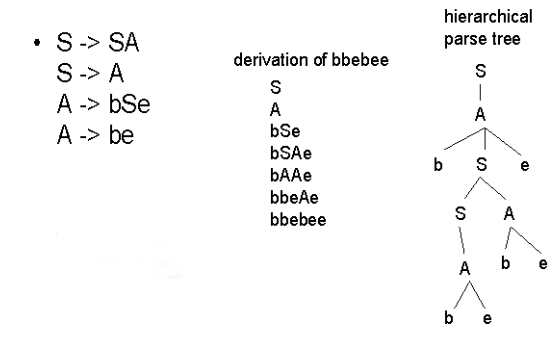
\includegraphics[width=0.7\textwidth]{img/GIC2.png}
    \caption{CFG example \protect\footnote{http://www.biiet.org/blog/wp-content/uploads/2013/07/img028.jpg}}
    \label{fig:CFG}
\end{figure}

%\footnote{http://www.biiet.org/blog/wp-content/uploads/2013/07/img028.jpg}
%falar dos terminais, nao terminais, start symbols e de Noam Chomsky

One valid sentences (Example in Figure ~\ref{fig:CFG}), could be : bbebee .

In the compilers area two major classes of grammars are used : CFG (Context-free grammar) and AG ( Attribute Grammar).

The difference between these two grammars are that a CFG is directed to define the syntax (only) and, AG contains semantic and syntax rules.

An AG is , basically, a GFC grammar extended with semantic definitions. It is a formal way to define attributes for the symbols that occur in each production of the underlying grammar. We can associate values to these attributes later, after processed with a parser; the evaluation will occur applying those semantic definition to any node of the abstract syntax tree.
These attributes are divided into two groups: synthesized attributes and inherited attributes.

The synthesized attributes are the result of the attribute evaluation rules for the root symbol of each subtree, and may also use the values of the inherited attributes. The inherited attributes are passed down from parent nodes to children or between siblings.

Like that it is possible to transport information anywhere in the abstract syntax tree which is one of the strength for using an AG (as seen on Listing ~\ref{lst:ag}).

%put an AG example !

\begin{comment}
\begin{figure}[h!]
  \centering
    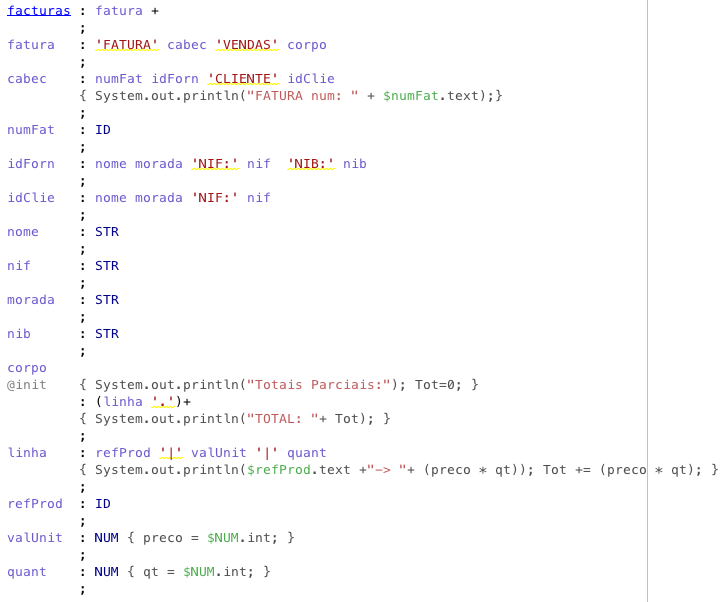
\includegraphics[width=0.9\textwidth]{img/ga.png}
    \caption{Example of an AG}
    \label{fig:GA}
\end{figure}
\end{comment}	

\begin{lstlisting}[caption={Example of an AG},label={lst:ag}]
facturas : fatura (facturas)*
         ;

fatura : 'FATURA' cabec 'VENDAS' corpo {System.out.println("Total Factura: "+$corpo.totOut);}
       ;

cabec : idFat idForn 'CLIENTE' idClie {System.out.println("Factura n: "+$idFat.text);}
      ;

idFat : numFat ;

numFat : ID ;

idForn : nome morada 'NIF:' nif 'NIB:' nib
       ;

idClie : nome morada 'NIF:' nif
       ;

nome :  STR ;

morada : STR;

nif : STR;

nib : STR;

corpo returns [int totOut]
    : linha '.' {$totOut += $linha.linhatot;}
      (linha '.' {$totOut += $linha.linhatot;})*
    ;

linha returns [int linhatot]
      : refProd '|' valUnit '|' quant {$linhatot = $valUnit.val * $quant.quan;System.out.println("Ref: "+$refProd.text+" Total linha: "+($linhatot)+" Euros");}
      ;
	
	refProd : ID;
valUnit returns [int val]
        : NUM {$val = $NUM.int;}
        ;
quant returns [int quan]
    : NUM {$quan = $NUM.int;}
    ;

\end{lstlisting}


In this way, an AG will be used to specify the translation from syntax tree directly into code for some specific machine or into another intermediate language.
For our thesis, the AG will be processed by ANTLR tool in order to build automatically the parser, the attribute evaluator, and the code generation.
%%%%%%%%%%%%%%%%%%%%%%%%%%%%%%%%%%%%%%%%%%%%%%%%%%%%%%

\section{Formal Grammar}
According to Noam Chomsky, a classic formalization of generative grammars is composed by:
\begin{itemize}
        \item A finite set N of nonterminals symbols.
        \item A finite set $\sum$  of terminals symbols.
        \item A finite set P of production rules.
        \item A start symbol S $\in$  P
\end{itemize}
A grammar is formally constructed by that tuple (N,$\sum$,P,S).



Grammar is a set of productions rules which describes the syntax of the language (not semantic). Each grammar has only one start symbol production that defines where the grammar begins.
%And there is two types after that the production rules are then applied in any order.
And each production is composed by two things : LHS (Left Hand Side) and RHS (Right and Side). Left Hand Side represents the non terminal and the right hand side represents the behaviour of the rule ( composed by non terminal and terminal).

\begin{lstlisting}[caption={A rule production},label={lst:ruleExample}]
     liss : 'program' identifier body
          ;
\end{lstlisting}

In ~\ref{lst:ruleExample}, we can see that it is composed by two sides. The left hand side and the right hand side, delimited by ':'.
On the LHS, 'liss' is a non-terminal and on the RHS, it is composed by the terminal 'program' followed by two non-terminals.
This is the syntax of one production rule of the grammar.

Now let's speak about the entire syntax of the LISS.

%\subsection{LISS Syntax}
\chapter{LISS language}

LISS ~\citep{CH07a} -that stands for Language of Integers, Sequences and Sets- is an imperative programming language, defined by the Language Processing members (Pedro Henriques and Leonor Barroca) at UM for teaching purposes (compiler course).

The idea behind the design of LISS language was to create a simplified version of the more usual imperative languages although combining functionalities from various languages.

It is designed to have atomic or structured integer values, as well as, control statements and block structure statements.

Now, let's explain in the next sections the basic statements of the language and its data types, using a context free gammar.

\section{LISS Data types}
\label{sec:data_types}

There are 5 types available.
From atomic to structured types, they are known as : integer, boolean, array, set and sequence.

Used for declaring a variable in a program, the data type gives us vital information for understanding what kind of value we are dealing with.

Let's obverse a LISS code example:

\begin{lstlisting}[caption={Declaring a variable in LISS},label={lst:declare_variable}]
  a -> integer;
  b -> boolean;
  c -> array size 5,4;
  d -> set;
  e -> sequence;
\end{lstlisting}

As we can see in Listing ~\ref{lst:declare_variable}, some variables ('a','b','c','d' and 'e')  are being declared each one associated to a type ('integer', 'boolean', 'array', 'set' and 'sequence').
Syntactically, in LISS, this is done by writing the variable name followed by an arrow and the type of the variable (see Listing ~\ref{lst:variable_declaration_BNF}).

\begin{lstlisting}[caption={CFG for declaring a variable in LISS},label={lst:variable_declaration_BNF}]
  variable_declaration : vars '->' type ';'
                     ;
  vars : var (',' var )*
     ;
  var : identifier value_var
    ;
  value_var :
          | '=' inic_var
          ;
  type : 'integer'
     | 'boolean'
     | 'set'
     | 'sequence'
     | 'array' 'size' dimension
     ;
  dimension : number (',' number )*
          ;
  inic_var : constant
         | array_definition
         | set_definition
         | sequence_definition
         ;
  constant : sign number
         | 'true'
         | 'false'
         ;
  sign :
     | '+'
     | '-'
     ;

\end{lstlisting}

Variables that are not initialized, have a default value (according to Table ~\ref{tbl:data_types}).

\begin{table}[]
\centering
\caption{LISS data types}
\label{tbl:data_types}
\begin{tabular}{|c|c|}
\hline
\textbf{Type}       & \multicolumn{1}{l|}{\textbf{Default Value}} \\ \hline
boolean             & false                                       \\ \hline
integer             & 0                                           \\ \hline
array               & {[}0,...,0{]}                               \\ \hline
set                 & \{\}                                        \\ \hline
sequence            & nil                                         \\ \hline
\end{tabular}
\end{table}

\newpage
Additionally, we may change the default values of the variables by initializing them with a different value (see an example in Listing ~\ref{lst:variable_declaration}).
This can be made by writing an equal symbol after the variable name and, then, inserting the right value according to the type (see example in Listing ~\ref{lst:variable_declaration_BNF}).

\begin{lstlisting}[caption={Initialize a variable},label={lst:variable_declaration}]
  a = 4, b -> integer;
  t = true -> boolean;
  vector1 = [1,2,3], vector2 -> array size 5;
  a = { x | x<10} -> set ;
  seq1 = <<10,20,30,40,50>>, seq3 = <<1,2>>, seq2 -> sequence;
\end{lstlisting}

Now, let's define which types are, correctly, associated with the arithmetic operators and functions in LISS (see Table ~\ref{tbl:type_operations}).


\begin{table}[]
\centering
\caption{Operations and signatures in LISS}
\label{tbl:type_operations}
\begin{tabular}{|c|c|}
\hline
\textbf{Operators \&\& Functions} & \multicolumn{1}{l|}{\textbf{Signatures}} \\ \hline
+ (add)                                   & integer x integer \verb+->+ integer                                        \\ \hline
- (subtract)                              & integer x integer \verb+->+ integer                                        \\ \hline
\verb+||+ (or)                            & boolean x boolean  \verb+->+ boolean                                       \\ \hline
++ (union)                                & set x set \verb+->+ set                                                    \\ \hline
/ (division)                              & integer x integer \verb+->+ integer                                        \\ \hline
* (multiply)                              & integer x integer \verb+->+ integer                                        \\ \hline
\&\& (and)                                & boolean x boolean \verb+->+ boolean                                        \\ \hline
** (intersection)                         & set x set \verb+->+ set                                                    \\ \hline
== (equal)                                & integer x integer \verb+->+ integer; boolean x boolean \verb+->+ boolean   \\ \hline
!= (not equal)                            & integer x integer \verb+->+ integer; boolean x boolean \verb+->+ boolean   \\ \hline
\textless  (less than)                    & integer x integer \verb+->+ boolean                                        \\ \hline
\textgreater  (greater than)              & integer x integer \verb+->+ boolean                                        \\ \hline
\textless= (less than or equal to)        & integer x integer \verb+->+ boolean                                        \\ \hline
\textgreater= (great than or equal to)    & integer x integer \verb+->+ boolean                                        \\ \hline
in (contains)                              & integer x set \verb+->+ boolean                                            \\ \hline
tail                                      & sequence \verb+->+ sequence                                                \\ \hline
head                                      & sequence \verb+->+ integer                                                 \\ \hline
cons                                      & integer x sequence \verb+->+ sequence                                      \\ \hline
delete                                    & integer x sequence \verb+->+ sequence                                      \\ \hline
copy                                      & sequence x sequence \verb+->+ void                                         \\ \hline
cat                                       & sequence x sequence \verb+->+ void                                         \\ \hline
isEmpty                                   & sequence \verb+->+ boolean                                                 \\ \hline
length                                    & sequence \verb+->+ integer                                                 \\ \hline
isMember                                  & integer x sequence \verb+->+ boolean                                       \\ \hline
\end{tabular}
\end{table}

\newpage

So, in Table ~\ref{tbl:type_operations}, we list the operators and functions, available in LISS, and their signature.
In order to understand the table better, we will explain how to read the table and its signature with one example.

Consider the symbol '+' (Table ~\ref{tbl:type_operations}), indicates that both operands must be of type integer.
The result of that operation, indicated by the symbol '\verb+->+', will be an integer.
%Notice that semantically, operations must be validated according to the table ~\ref{tbl:type_operations}, otherwise the operations would be incorrect and throw an error.
Semantically, operations must be valid according to Table ~\ref{tbl:type_operations}; otherwise the operations would be incorrect and throw an error.

\bigbreak

\textbf{Arrays.}
LISS supports a way of indexing a collection of integer values such that each value is uniquely addressed. LISS also supports an important property of multidimensionality.

Called as 'array', it is considered to be a static structured type due to the fact that its dimensions and maximum size of elements in each dimension is fixed at the declaration time.

%One of its, most important, property is that he may have multiple dimension.

The operations defined over arrays are:

\begin{enumerate}
\item \textit{indexing} %- denoted by '[' and ']', it selects the value of the chosen indexed array.
\item \textit{assignment} %- 
\end{enumerate}

%explaining probably indexing and assignment

Arrays can be initialized, in the declaration section, partially or completely in each dimension.
For example, consider an array of dimension 3x2 declared in the following way:

\begin{lstlisting}
  array1 = [[1,2],[5]] -> array size 3,2;
\end{lstlisting} 

Thi is equivalent to the initialization below:

\begin{lstlisting}
  array1 = [[1,2],[5,0],[0,0]] -> array size 3,2;
\end{lstlisting}

Notice that the elements that are not explicitly assigned, are initialized with the value 0 (see Table ~\ref{tbl:data_types}).

The grammar for array declaration and initialization is shown below.

\begin{lstlisting}
  array_definition : '[' array_initialization ']'
                 ;

  array_initialization : elem (',' elem)*
                     ;

  elem : number
     | array_definition
     ;
\end{lstlisting}

\bigbreak

\textbf{Sets.}
The type \textit{set}, in LISS, is a collection of integers with no repeated numbers.

It is defined by an expression, in a comprehension, instead of by enumeration of its element.
A \textit{set} variable can have an empty value and, syntactically, this is done by writing '\verb+{}+'.

To define a set by comprehension, the free variable and the expression shall be return between curly brackets. The 'identifier' (free variable) is separated from the expression by an explicit symbol '\verb+|+'. 

The expression is built up from relational and boolean operators to define an integer interval.

The operations defined for sets are :
\begin{enumerate}
\item \textit{union}
\item \textit{intersection}
\item \textit{in} (membership)
\end{enumerate}


Let's see an example of its syntax below:

\begin{lstlisting}
  set1 = {x | x < 6 && x > -7} -> set;
\end{lstlisting}

This declaration defines a set including all the integers from -7 to 6 (open interval) and others numbers are not included in the set.

The syntax for set declaration and initialization is :

\begin{lstlisting}
  set_definition : '{' set_initialization '}'
               ;

  set_initialization :
                   | identifier '|' expression
                   ;
\end{lstlisting}

\bigbreak

\textbf{Sequences.}
Considered as a dynamic array of one dimension, the type sequence is a list of ordered integers. But, in opposition to the concept of an array, its size is not fixed; this means that it grows dinamicallly at run time like a linked list.
A sequence can have the empty value (syntactically done by writing '\verb+<<>>+').
If not empty, the sequence value is defined by enumerating its components (integers) in the right order.
Let's see deeper with one example:

\begin{lstlisting}[caption={Example of valid operations using sequence on LISS},label={lst:sequence_example_use}]
  c=<<1,2,3>> -> sequence;
\end{lstlisting}

In the example of Listing ~\ref{lst:sequence_example_use} the sequence is defined by three numbers (3,2,1). 

The operations defined for the sequence are:
\begin{enumerate}
\item \textit{tail} (all the elements but the first)
\item \textit{head} (the first element of the sequence)
\item \textit{cons} (adds an element in the head of the sequence)
\item \textit{delete} (remove a given element from the sequence)
\item \textit{copy} (copies all the elements to another sequence)
\item \textit{cat} (concatenates the second sequence at the end of the first sequence)
\item \textit{isEmpty} (true if the sequence is empty)
\item \textit{length} (number of elements of the sequence)
\item \textit{isMember} (true if the number is an element of the sequence)
\end{enumerate}
Those operations will be explained further and deeper.

The grammar below defines how to declare a sequence:

\begin{lstlisting}
  sequence_definition : '<<' sequence_initialization '>>'
                    ;

  sequence_initialization :
                        | values
                        ;

  values : number (',' number )*
       ;

\end{lstlisting}

\subsection{LISS lexical conventions}

Once you've declared a variable of a certain type, you cannot redeclare it again with the same name.

The variable name must be unique (see Listing ~\ref{lst:variable_name_single}).

\begin{lstlisting}[caption={Conflicts with variable names},label={lst:variable_name_single}]
  program single_variable_name{
    declarations
      int=1 -> integer;
      int=true -> boolean; //cannot declare this variable with this name (already exists)
    statements
  }
\end{lstlisting}

Keywords cannot be used as variable names.

For example, you cannot declare a variable with the name \textit{array} due to the fact that \textit{array} is a keyword in LISS (in this case, a type).

See the example in Listing ~\ref{lst:keyword_reserved_name}.
\begin{lstlisting}[caption={Conflicts with keyword names},label={lst:keyword_reserved_name}]
  array -> array size 3,4; //variable 'array' cannot be declared as a name
  integer -> integer;
\end{lstlisting}

Variable names contain only letters and numbers, or the underscore sign. However the first character of the variable name must be a letter (lower or upper case).
See the example below:

\begin{lstlisting}[caption={},label={}]
  My_variable_1
  MyVariable1
\end{lstlisting}

Numbers are composed of digits (one or more). 
Nothing more is allowed.

See example below:

\begin{lstlisting}[caption={},label={}]
  1562
  1
\end{lstlisting}

A string is a sequence of n-characters enclosed by double quotes.

See example below:

\begin{lstlisting}[caption={},label={}]
  "This is a string"
\end{lstlisting}

\section{LISS blocks and statements}

A LISS program is always composed of two parts: declarations and statements (a program block).
LISS language is structured with a simple hierarchy.
And this is done by structuring LISS code as a block.

Any program begins with a name then appear the declaration of variables and subprograms. After that appear the flow of the program by writing statements.

Let's see one example (see Listing ~\ref{lst:block_liss}).

\begin{lstlisting}[caption={The structure of a LISS program (example)},label={lst:block_liss}]
  program sum{
    declarations
        int=2 -> integer;
    statements
        writeln(int+3);
  }
\end{lstlisting}

So a program in LISS begins by, syntactically, writing 'program' and then the name of the program (in this case, the name is 'sum').
A pair of curly braces delimits the contents of the program; that is done by opening it after the name of the program and closing it at the end of the program.
After the left brace, appear the declaration and statement blocks.

As in a traditional imperative language (let's compare 'C language'), if we don't take the habit of declaring the variable always in a certain part of the code, it becomes confusing. This makes the programmer's life harder to understand the code when the code is quite long.

So, in LISS, we always declare variables first (syntactically written by 'declarations')  and then the statements (syntactically written by 'statements').
This is due to the fact that LISS wants to help the user to create solid and correct code. And in this case, the user will always know that all the variable declarations will be always at the top of the statements and not randomly everywhere (see grammar in Listing ~\ref{lst:program_grammar}).

\begin{lstlisting}[caption={CFG for program in LISS},label={lst:program_grammar}]
  liss : 'program' identifier body
     ;

  body : '{'
       'declarations' declarations
       'statements'   statements
       '}'
     ;
\end{lstlisting}

\subsection{LISS declarations} \label{subsec:liss_declarations}
The declaration part is divided into two other parts: variable declarations and subprogram declarations, both optional.

The first part is explained in section ~\ref{sec:data_types}; the subprogram part will be discussed later in section ~\ref{sec:subprograms}.

This part is specified by the following grammar (see Listing ~\ref{lst:declarations_grammar}).

\begin{lstlisting}[caption={CFG for declarations in LISS},label={lst:declarations_grammar}]
  declarations : variable_declaration* subprogram_definition*
             ;
\end{lstlisting}

\subsection{LISS statements}

As said previously, under the statements part, we control and implement the flow of a LISS program.
In LISS, we may write none or, one or more statements consecutively.

Every statement ends with a semicolon, unless two type of statements (conditional and cyclic statements) as shown in Listing ~\ref{lst:liss_statements_bnf}.

\begin{lstlisting}[caption={CFG for statements in LISS},label={lst:liss_statements_bnf}]
  statements : statement*
           ;
  statement : assignment ';'
          | write_statement ';'
          | read_statement ';'
          | function_call ';'
          | conditional_statement
          | iterative_statement
          | succ_or_pred ';'
          | copy_statement ';'
          | cat_statement ';'
          ;
\end{lstlisting}

Let's see one example of a LISS program which shows how the language shall be used (see Listing ~\ref{lst:statements_example}).

\begin{lstlisting}[caption={Example of using statements in LISS},label={lst:statements_example}]
  program factorial{
    declarations
        res=1, i -> integer;
    statements
        read(i);
        for(j in 1..i){
            res=res*j;
        }
        writeln(res);
  }
\end{lstlisting}

\textbf{Assignment.} This statement assigns, as it is called, values to a variable and it is defined for every type available on LISS.
This operation is done by writing the symbol "=" in which a variable is assigned to the left side of the symbol and a value to the right side of the symbol.

Notice that an assignment requires that the variable on the left and the expression on the right must agree in type.

Let's see in Listing ~\ref{lst:assignment_example} an example.

\begin{lstlisting}[caption={Example of assignment in LISS},label={lst:assignment_example}]
  program assignment1{
    declarations
      intA -> integer;
      bool -> boolean;  
    statements
      intA = -3 + 5 * 9;
      bool = 2 < 8;
  }
\end{lstlisting}

In Listing ~\ref{lst:assignment_example}, we can see assignment statements of integers and boolean types.
Those assignments are correct, as noticed in the previous paragraphs, because they have the same type on the left and right side of the symbol equals (operations of integers assigned to a variable of integer type and operation of booleans assigned to a variable of boolean type).

The grammar that rules the assignment is shown at Listing ~\ref{lst:assignment_bnf}.

\begin{lstlisting}[caption={CFG for assignment in LISS},label={lst:assignment_bnf}]
  assignment : designator '=' expression
           ;
\end{lstlisting}

\textbf{I/O.} The input and output statements are also available in LISS.

The \textit{read} operations, called syntactically as 'input' in LISS, assign a value to a variable obtained from the standard input and require to be an atomic value (in this case, only an integer value).


\begin{lstlisting}[caption={Example of input operation in LISS}, label={lst:input_example}]
  program input1{
    declarations
      myInteger -> integer;
    statements
      input(myInteger);
  }
\end{lstlisting}

Notice that, in Listing ~\ref{lst:input_example}, the variable \textit{myInteger} must be declared  and must be integer otherwise the operations fails.
The grammar that rules the input statement, is shown in Listing ~\ref{lst:input_bnf}.

\begin{lstlisting}[caption={CFG for input operation in LISS}, label={lst:input_bnf}]
 read_statement : 'input' '(' identifier ')'
               ; 
\end{lstlisting}

The \textit{write} operations, called syntactically as 'write' or 'writeln' in LISS, print an integer value in the standard output.
Notice that 'write' operation only prints the value and doesn't move to a new line; instead, 'writeln' moves to a new line at the end.

Listing ~\ref{lst:output_example} shows some more examples.

\begin{lstlisting}[caption={Example of output operations in LISS},label={lst:output_example}]
  writeln(4*3);
  writeln(2);
  writeln();
\end{lstlisting}

Note that the write statement may have as assignment, an atomic value as well as an empty value or some complex arithmetic expression (see grammar in ~\ref{lst:output_bnf}).

\begin{lstlisting}[caption={CFG for output operation in LISS},label={lst:output_bnf}]
  write_statement : write_expr '(' print_what ')'
                ;

  write_expr : 'write'
           | 'writeln'
           ;

  print_what :
           | expression
           ;
\end{lstlisting}

\textbf{Function call.} The function call is a statement that is available for using the functions created in the program under the section 'declarations' (as described in Section ~\ref{subsec:liss_declarations}).
This will allow reusing functions that were created by calling them instead of creating duplicated code.

See Listing ~\ref{lst:call_function_example} for a complete example.

\begin{lstlisting}[caption={Example of call function in LISS},label={lst:call_function_example}]
 program SubPrg {

  declarations

    a = 4, b= 5, c= 5 -> integer;
    d = [10,20,30,40], ev -> array size 4;


    subprogram calculate() -> integer
    {
      declarations
            fac = 6 -> integer;
            res = -16 -> integer;

        subprogram factorial(n -> integer; m -> array size 4) -> integer
            {
              declarations
                    res = 1 -> integer;
              statements
                    while (n > 0)
                    {
                        res = res * n;
                        n = n -1;
                    }

                    for (a in 0..3) stepUp 1
                    {
                      d[a] = a*res;
                    }
                    return res;
            }
      statements
            res = factorial(fac,d);
            return res/2;
    }


  statements

    a = calculate();
    writeln(a);
    writeln(d);
}
\end{lstlisting}

In Listing ~\ref{lst:call_function_example}, we can see that the function \textit{calculate()}, called in the main program, and that is created under the declarations section.

The grammar who rules the function call is shown in Listing ~\ref{lst:call_function_bnf}.

\begin{lstlisting}[caption={CFG for call function in LISS},label={lst:call_function_bnf}]
  function_call : identifier '(' sub_prg_args ')'
              ;
  sub_prg_args :
             | args
             ;
  args : expression (',' expression )*
     ;

\end{lstlisting}

\subsection{LISS control statements}

LISS language includes some statements for controlling the execution flow at runtime with two different kind of behaviour.

The first one is called conditional statement and it has only one variant in LISS language (see Listing ~\ref{lst:control_statements}).

The second one is called cyclic statement or iterative statement, and it has two variants (see Listing ~\ref{lst:control_statements}).

\begin{lstlisting}[caption={CFG for control statement in LISS},label={lst:control_statements}]
  conditional_statement : if_then_else_stat
                      ;
  iterative_statement : for_stat
                    | while_stat
                    ;
\end{lstlisting}

These control statements, mimics the syntax and the behaviour  of other modern imperative language.

\paragraph{Conditional}

The if-statement, which is common across many modern programming languages, performs different actions according to decision depending on the truth value of a control conditional expression: an alternative 'else' block is also allowed (optional).

If the conditional expression evaluates 'true', the content of 'then' block will be executed. Otherwise, if the condition is 'false', the 'then' block is ignored; and if an 'else' block is provided it will be executed alternatively.

Let's see an example in Listing ~\ref{lst:if_program}.

\begin{lstlisting}[caption={LISS syntax of a if statement},label={lst:if_program}]
  if(y==x)
  then{
    x=x+1;
  }else{
    x=x+2;
  }
\end{lstlisting}

The code shown in Listing ~\ref{lst:if_program}, means that the if-statement evaluates the conditional expression 'y==x'.
If the expression, which must be boolean, is true, then every action in the 'then' block will be executed and the block 'else' will be ignored.
Otherwise, if the condition is false, every action in the 'else' block is executed ignoring the 'then' block.

If the else-statement is not provided, the if-statement will finish and do not perform any actions.


The syntax of the if-statement in LISS is shown in Listing ~\ref{lst:if_bnf}.



\begin{lstlisting}[caption={CFG for iterative statement in LISS},label={lst:if_bnf}]
  if_then_else_stat : 'if' '(' expression ')'
                    'then' '{' statements '}'
                    else_expression
                    ;

  else_expression :
                | 'else' '{' statements '}'
                ;
\end{lstlisting}

\paragraph{Iterative}

We should take a look at the behaviour of each iterative control statement to understand it deeper.

The  for-statement offers two variants to control the repetition.
Normally, in a conventional way, the for-loop has a control variable which takes a value in a given range and step up or step down by a default or an explicit value.

In LISS, the control variable is set in a given integer interval defined by the lower and upper bounds. By default, the step is one, which means that the control variable is incremented by one at the end of each iteration but it is possible to increment or decrement it by a different value, setting it explicitly.
Additionally, we may write a condition for filtering the values in the interval.
This can be done as shown in the following example:
\begin{lstlisting}[caption={LISS syntax of a for-loop statement},label={lst:for-loop}]
  for(a in 1..10) stepUp 2 satisfying elems[a]==1{
	  ...
  }
\end{lstlisting}
In Listing ~\ref{lst:for-loop}, the control variable 'a' is set to a range 1 to 10 and would be increased (due to the 'stepUp' constructor) by 2. Also there is a filter condition (after the 'satisfying' keyword) that restricts the values of 'a' to those that makes the condition 'elems[a]==1' true. Notice that the filter expression must be boolean. 

After each cycle, the control variable will be incremented with value 2 and the filter condition tested again. 

This is the first way of expressing the control in a for-loop statement. Let's see the second way in the sequel.

There is also the possibility to assign to the control variable the values in an array, like illustrated in the following example:

\begin{lstlisting}[caption={LISS syntax of a for-each statement on array},label={lst:for-each_array}]
  for(b inArray elems){
       	...
  }
\end{lstlisting}
In Listing ~\ref{lst:for-each_array}, the control variable  'b' is assigned with all of the elements of the array and begins with his lower index (zero) until his upper index (size of the array minus one).
Notice that, in this case, we cannot apply an increment or decrement neither a filter condition.

The next grammar fragment describes the cycle 'for' in LISS:

\begin{lstlisting}[caption={CFG for for-statement in LISS}]
  for_stat : 'for' '(' interval ')' step satisfy
           '{' statements '}'
         ;
  interval : identifier type_interval
         ;
  type_interval : 'in' range
              | 'inArray' identifier
              ;
  range : minimum '..' maximum
      ;
  minimum : number
        | identifier
        ;
  maximum : number
        | identifier
        ;
  step :
     | up_down number
     ;
  up_down : 'stepUp'
        | 'stepDown'
        ;
  satisfy :
        | 'satisfying' expression
        ;
\end{lstlisting}

%write the for statetement with step and satisfy explication

Finally, the while-statement consists in a block of code that is executed repeatly until the control condition evaluates 'false'. 

Each time that the 'while' block is performed, the conditional expression associated will be evaluated again to decide whether to repeat the execution of the statements in the block or to continue the normal program flow.

Let's see an example in Listing ~\ref{lst:while_program}.

\begin{lstlisting}[caption={LISS syntax of a while-statement in LISS},label={lst:while_program}]
  while (n > 0)
  {
    res = res * n;
    pred n;
  }
\end{lstlisting}

In Listing ~\ref{lst:while_program}, the while-statement is controled by the conditional expression '\verb+n>0+' that is evaluated at the beginning. If the condition is true, then all the actions that are inside the braces will be performed. Later, after executing all the actions, the condition will be evaluated again. If the condition remains 'true', then those actions would be executed again otherwise if the condition is false, the while-statement will be exited.

The syntax that rule the while-statement is shown below:

\begin{lstlisting}[caption={CFG for while-statement in LISS}]
  while_stat : 'while' '(' expression ')'
             '{' statements '}'
             ;
\end{lstlisting}



\subsection{Others statements}

LISS language offers other statements to make it more expressive easing the codification of any imperative algorithm.

\textbf{Succ/Pred.} Those statements are available for incrementing or decrementing a variable. This is a common situation in modern programming languages, making life easier for the developers. 

The keyword 'succ' means increment (successor) and the syntax 'pred' means decrease (predecessor). Only integer variables can be used with those constructors.

Listing ~\ref{lst:succ_or_pred_example} illustrates both statements.

\begin{lstlisting}[caption={Example of using succ/pred in LISS}, label={lst:succ_or_pred_example}]
  succ int1;
  pred int1;
\end{lstlisting}

As we can see in Listing ~\ref{lst:succ_or_pred_example}, variable 'int1' is, first, incremented by 1 and then it is decremented also by 1.

Grammar of 'succ' and 'pred' in LISS is shown in Listing ~\ref{lst:succ_or_pred_bnf}.


\begin{lstlisting}[caption={CFG for succ and pred in LISS}, label={lst:succ_or_pred_bnf}]
  succ_or_pred : succ_pred identifier
             ;
  succ_pred : 'succ'
          | 'pred'
          ;
\end{lstlisting}

\textbf{Copy statement.}
This statement is applied only to variables of type sequence.
Basically, it copies one sequence to another sequence.
Let's see an example in Listing ~\ref{lst:copy_example}.

\begin{lstlisting}[caption={Example of copy statement in LISS},label={lst:copy_example}]
  copy(seq1,seq2);
\end{lstlisting}

Notice that 'copy' is a statement and not a function: it modifies the arguments but does not return any value.

In Listing ~\ref{lst:copy_example}, the statement 'copy' copies the content of the variable \textit{seq1} to \textit{seq2}.

The grammar for 'copy' statement is in Listing ~\ref{lst:copy_bnf}.

\begin{lstlisting}[caption={CFG for copy statement in LISS},label={lst:copy_bnf}]
  copy_statement : 'copy' '(' identifier ',' identifier ')'
                 ;
\end{lstlisting}

\textbf{Cat statement.}

'Cat' statement is simular to 'copy', it only operates with variables of type sequence.
The behaviour of this statement is to concatenate a sequence to another sequence.
Let's see an example in Listing ~\ref{lst:cat_example}).

\begin{lstlisting}[caption={Example of cat statement in LISS},label={lst:cat_example}]
  cat(seq1,seq2);
\end{lstlisting}

In Listing ~\ref{lst:cat_example}, 'cat' concatenates the content of \textit{seq2} to \textit{seq1}.
Again, 'cat' is not a function; it modifies the arguments instead of returning a value.

The grammar for cat-statement is shown in Listing ~\ref{lst:cat_bnf}.

\begin{lstlisting}[caption={CFG for cat statement in LISS},label={lst:cat_bnf}]
  cat_statement : 'cat' '(' identifier ',' identifier ')'
                ;
\end{lstlisting}

\section{LISS subprograms}
\label{sec:subprograms}

In LISS, it is possible to organize the code by splitting the general block of statements into sub-programs. This allows the programmer to reuse or to give more clarity to his code by creating functions or procedures.
Also, it is possible to create sub-programs inside sub-programs by using a nesting strategy.

The syntax that defines a sub-program in LISS is shown in Listing ~\ref{lst:block_structure}.

\begin{lstlisting}[caption={CFG for block structure in LISS},label={lst:block_structure}]
  subprogram_definition: 'subprogram' identifier '(' formal_args ')' return_type f_body
                     ;
  f_body : '{'
         'declarations' declarations
         'statements' statements
         returnSubPrg
         '}'
       ;
  formal_args :
            | f_args
            ;
  f_args  : formal_arg (',' formal_arg )*
        ;
  formal_arg : identifier '->' type
           ;
  return_type :
            | '->' typeReturnSubProgram
            ;
  returnSubPrg :
             | 'return' expression ';'
             ;
\end{lstlisting}

Note that every variable declared inside of a sub-program is local, and it can be accessed only by other nested sub-programs.
However, variables declared in the program (not in a sub-program) are considered global and can be accessed by any sub-program. The usual scope rules are applied to LISS.

As can be inferred from the syntax above (Listing ~\ref{lst:block_structure}), the body of a sub-program is identical to the body of a program --- the same declarations can be made and similar statements can be used.










%Also, in LISS language, variables are declared firstly and then we may code the program.
%Notice that this restriction is done for a better experience of the programmer. 
%This means that variables must be declared always on top of the program before they will be used on the rest of the program.


%It allows handling integers, sets of integers, dynamic sequences, complex numbers, polynomials, etc., etc~\citep{CH07d,CH07a,CH06a,CH06b,CH05a}.


\newpage


%write appendix , code gic liss

\section{Evolution of LISS syntax}
Due to the maturity of the language already done along the years, we have added some few but extra changes for a better experience of the programming language.
%The syntax of the LISS language (Figure ~\ref{lst:GIC_LISS} ), has been constructed with ANTLR which is ANother Tool for Language Recognition where it collaborates with the Java platform.

%One of the first objectives is that we have changed the format of the syntax. We have translated the old LISS language to a brand new extended BNF format (as shown in Figure ~\ref{lst:GIC_LISS}).

One of the first changes was concerned with declarations in order to avoid mixing functions and variable declarations.
We, indirectly, teach the programmer by doing it in the right way. So we declare, first, the variables and then the functions.
\begin{lstlisting}[caption={},label={lst:declaration_LISS}]
declaration : variable_declaration * subprogram_definition *
            ;
\end{lstlisting}

Another change was to add punctuation after each statement (see Figure ~\ref{lst:statement_LISS}).
\begin{lstlisting}[caption={Function statement},label={lst:statement_LISS}]
statement : assignment  ';'
          | write_statement  ';'
          | read_statement  ';'
          | conditional_statement
          | iterative_statement
          | function_call ';'
          | succ_or_pred  ';'
          | copy_statement  ';'
          | cat_statement  ';'
          ;
\end{lstlisting}

Another change was adding also a 'cat\_statement' rule which works with only sequences. It concatenates a sequence with another sequence.

Regarding arrays, it was previously possible to use any expression to access elements of the array. So it was possible to index with a boolean expression what does not make any sense.
Now only integers are allowed (see in Listing ~\ref{lst:elem_array_LISS}).


\begin{lstlisting}[caption={Rule element of array},label={lst:elem_array_LISS}]
elem_array : single_expression (',' s2=single_expression )*
           ;
\end{lstlisting}

In the previous version of LISS, it was allowed to create a boolean expression associating relational operators, but we decided to change that and not permit associativity; only able to create one boolean expression (see Listing ~\ref{lst:expression_LISS}).
It does not make sense to have an expression like that : '3 == 4 == 5 != 6'.
\begin{lstlisting}[caption={Rule for Boolean expression},label={lst:expression_LISS}]
expression : single_expression (rel_op single_expression )?
           ;
\end{lstlisting}

We added the possibility of using parenthesis on expressions (see Listing ~\ref{lst:factor_LISS}).

\begin{lstlisting}[caption={Rule factor},label={lst:factor_LISS}]
factor: '(' expression ')'
      ;
\end{lstlisting}

We changed the rules of two pre-defined functions: 'cons' and 'del'. These functions were working both in the same way. Waiting for an expression and a variable as arguments. Now, we decide to change that allowing to expression as arguments giving more expressive power to those functions (see Listing ~\ref{lst:cons_del_LISS}).

\begin{lstlisting}[caption={Rule cons and delete},label={lst:cons_del_LISS}]
cons // integer x sequence -> sequence
     : 'cons' '(' expression ',' expression ')'
     ;

delete // del : integer x sequence -> sequence
       : 'del' '(' expression ',' expression ')'
       ;
\end{lstlisting}

Besides adding some improvements to the grammar, we additionally deleted a rule which we thought not necessary to control the for-statement (see Listing ~\ref{lst:type_interval_LISS}).
\begin{lstlisting}[caption={Rule type interval},label={lst:type_interval_LISS}]
type_interval : 'in' range
              | 'inArray' identifier
              //| 'inFunction' identifier
              ;
\end{lstlisting}

Last but not least, we also added comments to the programming language, giving more power to the programmer.

\begin{lstlisting}[caption={Lexical rule for Comment},label={lst:comments_LISS}]
fragment
COMMENT
    : '/*'.*?'*/' /* multiple lines comment*/
    | '//'~('\r' | '\n')* /* single line comment*/
    ;
\end{lstlisting}











\chapter{Target machine: MIPS}

%\section{MIPS}

MIPS, from Microprocessor without Interlocked Pipeline Stages, is a Reduced Instruction Set Computer (RISC) developed by MIPS Technologies. 
Born in 1981, a team led by John L. Hennessy at Stanford University began to work on the first MIPS processor.

The main objective for creating MIPS, was to increase performance with deep instructions pipelines, a main problem back to the 80's. 
Some instructions, as division, would take a longer time to complete due to the fact that CPU needed to wait that the division ended before passing to the next instruction into the pipeline.

As MIPS solved those problems, it was primarly used for embedded systems and video games consoles (which requires a lot of arithmetic computation). 
% until late 2006, when it came to computers.

Now, the architecture of MIPS, along the years, has gained maturity and provides different versions of it (MIPS32, MIPS64....) \footnote{according to wikipedia \url{https://en.wikipedia.org/wiki/MIPS_instruction_set}}.

Figure ~\ref{fig:MIPSarchitecture} illustrate the architecture of MIPS.

%The architecture of MIPS is composed by 5 stages (see Figure ~\ref{fig:MIPSarchitecture}).

\begin{figure}[h!]
  \centering
    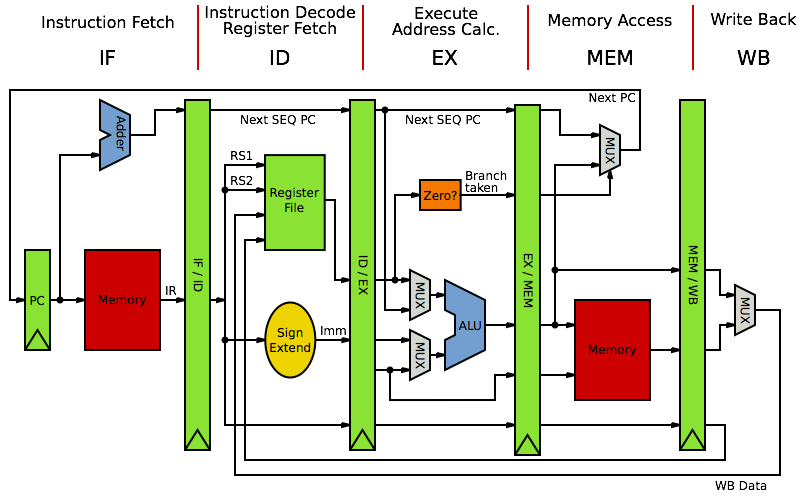
\includegraphics[width=1\textwidth]{img/MIPSarchitecture.png}
    \caption{MIPS architecture \protect\footnote{http://upload.wikimedia.org/wikipedia/commons/thumb/e/ea/MIPS\_Architecture(Pipelined).svg/300px-MIPS\_Architecture\_(Pipelined).svg.png}}
    \label{fig:MIPSarchitecture}
\end{figure}

%\protect\footnote{http://upload.wikimedia.org/wikipedia/commons/thumb/e/ea/MIPS_Architecture_(Pipelined).svg/300px-MIPS_Architecture_(Pipelined).svg.png}

\newpage

In this chapter, we will talk about all the architecture of MIPS with the 32-bit version.

\section{MIPS coprocessors}

MIPS was born for solving complex arithmetic problems by reducing the consuming time in those operations.

And this is done by the implementation of coprocessors with MIPS.

The MIPS architecture defines four coprocessors designed, respectively, CP0, CP1, CP2 and CP3:

\begin{enumerate}
\item Coprocessor 0, denoted by ~\textit{CP0}, is incorporated on the CPU chips, it supports the virtual memory system and exception handling (also known as the ~\textit{System Control Coprocessor}).
\item Coprocessor 1, denoted by ~\textit{CP1}, is reserved the floating point coprocessor.
\item Coprocessor 2, denoted by ~\textit{CP2}, is reserved for specific implementations.
\item Coprocessor 3, denoted by ~\textit{CP3}, is reserved for the implementations of the architecture.
\end{enumerate}

Notice that coprocessor - ~\textit{CP0}, translates virtual addresses into physical addresses, manages excpetions, and handles switch between kernel, supervisor and user modes.

\section{MIPS cpu data formats}

The CPU of MIPS defines different formats:
\begin{itemize}
\item ~\textit{Bit} (1 bit, b)
\item ~\textit{Byte} (8 bits, B)
\item ~\textit{Halfword} (16 bits, H)
\item ~\textit{Word} (32 bits, W)
\end{itemize}




\section{MIPS compiler register usage}

MIPS architecture has 32 registers dedicated and there are some conventions to use those registers correctly.
Table ~\ref{tbl:compiler_register_usage} summarizes those registers, and their usage.


\begin{table}[h!]
\centering
\caption{MIPS registers}
\label{tbl:compiler_register_usage}
\begin{tabular}{cllc}
\hline
\multicolumn{1}{|c|}{\textbf{Name}} & \multicolumn{1}{c|}{\textbf{Number}} & \multicolumn{1}{c|}{\textbf{Use}}                                                                                                           & \multicolumn{1}{c|}{\textbf{\begin{tabular}[c]{@{}c@{}}Callee must\\  preserve?\end{tabular}}} \\ \hline
\multicolumn{1}{|c|}{\$zero}        & \multicolumn{1}{l|}{\$0}             & \multicolumn{1}{l|}{has constant 0}                                                                                                         & \multicolumn{1}{c|}{No}                                                                        \\ \hline
\multicolumn{1}{|c|}{\$at}          & \multicolumn{1}{l|}{\$1}             & \multicolumn{1}{l|}{register reserved for assembler (temporary)}                                                                            & \multicolumn{1}{c|}{No}                                                                        \\ \hline
\multicolumn{1}{|c|}{\$v0 - \$v1}     & \multicolumn{1}{l|}{\$2 - \$3}         & \multicolumn{1}{l|}{\begin{tabular}[c]{@{}l@{}}register reserved for values for function returns\\  and expression evaluation\end{tabular}} & \multicolumn{1}{c|}{No}                                                                        \\ \hline
\multicolumn{1}{|c|}{\$a0 - \$a3}     & \multicolumn{1}{l|}{\$4 - \$7}         & \multicolumn{1}{l|}{registers reserved for function arguments}                                                                              & \multicolumn{1}{c|}{No}                                                                        \\ \hline
\multicolumn{1}{|c|}{\$t0 - \$t7}     & \multicolumn{1}{l|}{\$8 - \$15}        & \multicolumn{1}{l|}{temporary registers}                                                                                                  & \multicolumn{1}{c|}{No}                                                                        \\ \hline
\multicolumn{1}{|c|}{\$s0 - \$s7}     & \multicolumn{1}{l|}{\$16 - \$23}       & \multicolumn{1}{l|}{saved temporary registers}                                                                                            & \multicolumn{1}{c|}{Yes}                                                                       \\ \hline
\multicolumn{1}{|c|}{\$t8 - \$t9}     & \multicolumn{1}{l|}{\$24 - \$25}       & \multicolumn{1}{l|}{temporary registers}                                                                                                  & \multicolumn{1}{c|}{No}                                                                        \\ \hline
\multicolumn{1}{|c|}{\$k0 - \$k1}     & \multicolumn{1}{l|}{\$26 - \$27}       & \multicolumn{1}{l|}{register reserved for OS kernel}                                                                                        & \multicolumn{1}{c|}{N/A}                                                                       \\ \hline
\multicolumn{1}{|c|}{\$gp}          & \multicolumn{1}{l|}{\$28}            & \multicolumn{1}{l|}{global pointer}                                                                                                         & \multicolumn{1}{c|}{Yes}                                                                       \\ \hline
\multicolumn{1}{|c|}{\$sp}          & \multicolumn{1}{l|}{\$29}            & \multicolumn{1}{l|}{stack pointer}                                                                                                          & \multicolumn{1}{c|}{Yes}                                                                       \\ \hline
\multicolumn{1}{|c|}{\$fp}          & \multicolumn{1}{l|}{\$30}            & \multicolumn{1}{l|}{frame pointer}                                                                                                          & \multicolumn{1}{c|}{Yes}                                                                       \\ \hline
\multicolumn{1}{|c|}{\$ra}          & \multicolumn{1}{l|}{\$31}            & \multicolumn{1}{l|}{return address}                                                                                                         & \multicolumn{1}{c|}{N/A}                                                                       \\ \hline
\multicolumn{4}{l}{\textit{Note: N/A (Not applicable)}}                                                                                                                                                                                                                                                                  
\end{tabular}
\end{table}

The Table ~\ref{tbl:compiler_register_usage} is composed of 4 columns:

\begin{enumerate}
\item \textit{Name} column refers to the nomenclature of the register available in MIPS. Those will be used to interact with the instructions available in MIPS.
\item \textit{Number} column defines the number of each register. This number can also be used to refer to the register in an instruction.
\item \textit{Use} column refers to the meaning/definition of each register.
\item \textit{Callee must preserve?} column  provides information about the volatility of the register (used when a function is called).

\end{enumerate}

Also, beside of those 32 registers, 3 registers are dedicated to the CPU.

And they are known by:

\begin{itemize}

\item \textit{PC} - Program Counter register
\item \textit{HI} - Multiply and Divide register higher result
\item \textit{LO} - Multiply and Divide register lower result

\end{itemize}


\textit{PC} is the register which holds the address of the instruction that is being executed at the current time; ~\textit{HI} and ~\textit{LO} registers has different context whenever the instruction is being executed.
In this case, let's see what context they have:
\begin{itemize}
\item when there is a multiply (~\textit{mul} instruction) operation, the \textit{HI} and  ~\textit{LO}  registers store the result of integer multiply.
\item when there is a multiply-add (~\textit{madd} instruction) or multiply-subtract (~\textit{msub} instruction) operation, the ~\textit{HI} and ~\textit{LO} register store the result of integer multiply-add or multiply-subtract.
\item when there is a division (~\textit{div} instruction) operation, the ~\textit{HI} register store the remainder of the division and the ~\textit{LO} register store the quotient of the division operation.
\item when there is a multiply-accumulate (~\textit{} instruction) operation, the ~\textit{HI} and ~\textit{LO} registers store the accumulated result of the operation.
\end{itemize}

See an overview of the MIPS registers in Figure ~\ref{fig:MIPS_register}.

\begin{figure}[h!]
  \centering
    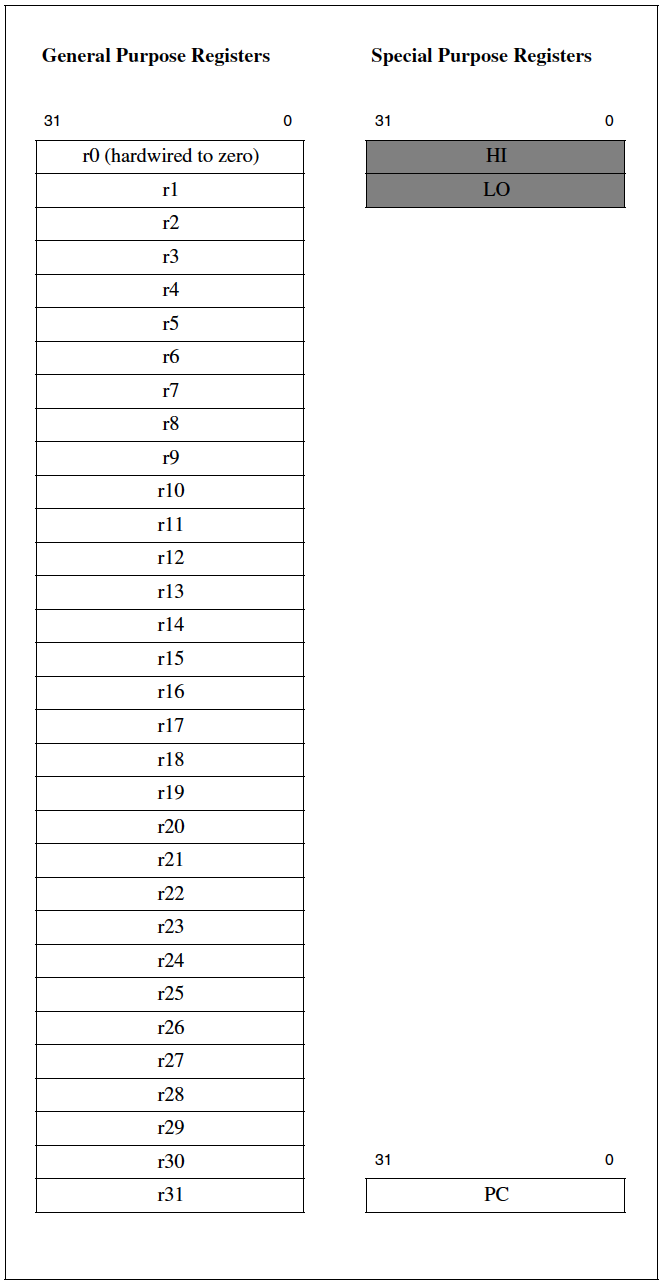
\includegraphics[scale=0.91]{img/mips_register.png}
    \caption{MIPS register}
    \label{fig:MIPS_register}
\end{figure}

\newpage



\section{MIPS instruction formats}
\label{sec:instruction_formats_mips}

Instructions, in MIPS, are divided into three types:
\begin{itemize}
\item R-Type
\item I-Type
\item J-Type
\end{itemize}

Each instruction is denoted by an unique mnemonic that represents the correspondent low-level machine instruction or operation.

Next sections provide the necessary details.

\subsection{MIPS R-Type}

R-Type instruction refers a register type instruction (it is the most complex type in MIPS).
The idea behind that instruction is to operate with registers only.

This type has the following format, mostly, in MIPS (see Listing ~\ref{lst:r-type_format}).

\begin{lstlisting}[caption={R-Type instruction format},label={lst:r-type_format}]
  OP rd, rs, rt
\end{lstlisting}

In Listing ~\ref{lst:r-type_format}, the instruction is composed of one mnemonic, denoted by \textit{OP}, and three operands, denoted by ~\textit{rd} (destination register), ~\textit{rs} (source register), ~\textit{rt} (another source register).

The R-Type instruction format as the following mathematical semantics:

\begin{lstlisting}[caption={},label={}]
  rd = rs OP rt
\end{lstlisting}

To understand better this instruction, let's see an example of one R-Type instruction in MIPS (see Listing ~\ref{lst:example_r-type}).

\begin{lstlisting}[caption={Example of a R-Type instruction},label={lst:example_r-type}]
  add $t1, $t1, $t2
\end{lstlisting}

The instruction shown in Listing ~\ref{lst:example_r-type} means that register \$t1 shall be added (due to \textit{add} mnemonic) to register \$t2 and their sum (the result) stored in register \$t1.

The following equivalence explains that meaning.

\begin{align*}
  OP\ rd,\ rs,\ rt &\iff rd\ =\ rs\ OP\ rt\\
  &\makebox[\widthof{${}={}$}]{$\Downarrow$} \\
  add\ \$t1,\ \$t1,\ \$t2 &\iff \$t1\ =\ \$t1\ add\ \$t2 \\
  &\makebox[\widthof{${}={}$}]{$\Downarrow$} \\
  \$t1\ &=\ \$t1\ +\ \$t2
\end{align*}

Table ~\ref{tbl:r-type_binary_machine_code} defines the bit-structure of a R-Type instruction in a 32-bit machine.

\begin{table}[h!]
\centering
\caption{R-Type binary machine code}
\label{tbl:r-type_binary_machine_code}
\begin{tabular}{|c|c|c|c|c|c|}
\hline
\textbf{opcode} & \textbf{rs} & \textbf{rt} & \textbf{rd} & \textbf{shift (shamt)} & \textbf{funct} \\ \hline
6 bits          & 5 bits      & 5 bits      & 5 bits      & 5 bits                & 6 bits         \\ \hline
\end{tabular}
\end{table}

Let's explain each of the columns in Table ~\ref{tbl:r-type_binary_machine_code}.

\begin{itemize}
\item \textbf{opcode}  defines the instruction type. For every R-Type instruction, \textit{opcode} is set to the value 0. The \textit{opcode} field is 6 bits long (bit 31 to bit 26).
\item \textbf{rs} this is the first source register; it is the register where it will load the content of the register to the operation.The \textit{rs} field is 5 bits long (bit 25 to bit 21).
\item \textbf{rt} this is the second source register (same behaviour as \textit{rs} register). The \textit{rt} field is 5 bits long (bit 20 to bit 16).
\item \textbf{rd} this is the destination register; it is the register where the results of the operation will be stored. The \textit{rd} field is 5 bits long (bit 15 to bit 11).
\item \textbf{shift amount} the amount of bits to shift for shift instructions. The \textit{shift} field is 5 bits long (bit 10 to bit 6).
\item \textbf{function} specify the operation in addition to the \textit{opcode} field. The \textit{function} field is 6 bits long (bit 5 to bit 0).

\end{itemize}

Let's see an example of a R-Type instruction and its transformation to machine code in Table ~\ref{tbl:r-type_transformation2machine_code}.


\newpage

\begin{align*}
  add\ \$t0,&\ \$t0,\ \$t1\\
  &\makebox[\widthof{${}={}$}]{$\Downarrow$} \\
  add\ \$8,&\ \$8,\ \$9\\
  &\makebox[\widthof{${}={}$}]{$\Downarrow$} \\
  (8)_{10}\ =&\ (01000)_{2}\\
  (9)_{10}\ =&\ (01001)_{2}\\
  add\ instruction\ (fu&nct\ field)\ =\ (100000)_{2}\\
  &\makebox[\widthof{${}={}$}]{$\Downarrow$}
\end{align*}

\vspace{-7mm}
\begin{table}[h!]
\centering
\begin{tabular}{|l|l|l|l|l|l|}
\hline
\textbf{opcode (6bits)}      & \textbf{rs (5bits)}        & \textbf{rt (5bits)}        & \textbf{rd (5bits)}        & \textbf{shift (shamt) (5bits)} & \textbf{funct (6bits)}     \\ \hline
\multicolumn{1}{|c|}{000000} & \multicolumn{1}{c|}{01000} & \multicolumn{1}{c|}{01001} & \multicolumn{1}{c|}{01000} & \multicolumn{1}{c|}{00000}     & \multicolumn{1}{c|}{100000} \\ \hline
\end{tabular}
\caption{Transformation of R-Type instruction to machine code}
\label{tbl:r-type_transformation2machine_code}
\end{table}

In Table ~\ref{tbl:r-type_transformation2machine_code}, the instruction 'add \$t0, \$t0, \$t1' will be normalized with the name of the register according to the number associated for the register in MIPS (see Table ~\ref{tbl:compiler_register_usage}). Then we do some operations for the two numbers (~\textit{8} and ~\textit{9}), we translate them as a binary number with 5 bits long. Also we give the information for the ~\textit{add} instruction, which is set for the MIPS architecture (not predictable).


After that, we complete the table for R-Type instruction according to Table ~\ref{tbl:r-type_binary_machine_code} with the informations available and the restriction/rules associated to R-Type instruction in MIPS.

Notice that the ~\textit{opcode} field for R-Type instruction are set to the value 0 (according to the explanation from Table ~\ref{tbl:r-type_binary_machine_code}).

Finally, we have our binary machine code for the instruction 'add \$t0, \$t0, \$t1' in Table ~\ref{tbl:r-type_transformation2machine_code}.

\subsection{MIPS I-Type}

I-Type instruction is an instruction which operate with an immediate value and a register value. 

Several different Immediate (~\textit{I-Type}) instructions formats are available.

Let's see those diferents formats for this type in Table ~\ref{tbl:I-Type_instruction_format}.

\begin{table}[h!]
\centering
\begin{tabular}{ccccll}
\multicolumn{1}{l|}{31 -- 26} & \multicolumn{1}{l|}{25 ---- 21} & \multicolumn{1}{l|}{20 -- 16} & \multicolumn{1}{l|}{15 -------- 11} & \multicolumn{1}{l|}{10 ------- 6} & 5 ----- 0                     \\ \hline
\multicolumn{1}{|c|}{opcode}  & \multicolumn{1}{c|}{rs}         & \multicolumn{1}{c|}{rt}       & \multicolumn{3}{c|}{immediate}                                                                          \\ \hline
\multicolumn{1}{|c|}{opcode}  & \multicolumn{1}{c|}{rd}         & \multicolumn{4}{c|}{offset}                                                                                                             \\ \hline
\multicolumn{1}{|c|}{opcode}  & \multicolumn{5}{c|}{offset}                                                                                                                                               \\ \hline
\multicolumn{1}{|c|}{opcode}  & \multicolumn{1}{c|}{rs}         & \multicolumn{1}{c|}{rt}       & \multicolumn{1}{c|}{rd}             & \multicolumn{2}{c|}{offset}                                       \\ \hline
\multicolumn{1}{|c|}{opcode}  & \multicolumn{1}{c|}{base}       & \multicolumn{1}{c|}{rt}       & \multicolumn{2}{c|}{offset}                                             & \multicolumn{1}{c|}{function} \\ \hline
\multicolumn{1}{l}{}          & \multicolumn{1}{l}{}            & \multicolumn{1}{l}{}          & \multicolumn{1}{l}{}                &                                   &                              
\end{tabular}
\caption{Distinct I-Type instruction formats}
\label{tbl:I-Type_instruction_format}
\end{table}

\newpage

In Table ~\ref{tbl:I-Type_instruction_format}, there are 5 differents instruction formats which explains the structure of the bits for every instruction.

The most frequent MIPS I-Type instruction is the first one, denoted as Imm16 (Immediate instruction with 16 bits immediate value), is used for logical operands, arithmetic signed operands, load/store address byte offsets and PC-relative branch signed instruction displacements (see Table ~\ref{tbl:imm16_instruction}).

\begin{table}[h!]
\centering
\begin{tabular}{l|l|l|l}
31 --- 26                    & 25 --- 21               & 20 --- 16               & 15 ----------------- 0         \\ \hline
\multicolumn{1}{|c|}{opcode} & \multicolumn{1}{c|}{rs} & \multicolumn{1}{c|}{rt} & \multicolumn{1}{c|}{immediate} \\ \hline
\end{tabular}
\caption{Immediate (I-Type) Imm16 instruction format}
\label{tbl:imm16_instruction}
\end{table}

Let's see examples of Imm16 instruction:

\begin{lstlisting}
  addi $t0, $t0, 10 // Arithmetic operation
  ori $t0, $t1, 5   // Logical operation
  beq $t0, $t1, 1    // Conditional branch operation
  lw $t0, array1($t0) //Data transfer operation
\end{lstlisting}

The second instruction, denoted as Immediate Off21 instruction (Immediate instruction with 21bits offset), is used for comparing a register against zero and branch (offset field is larger than the usual 16-bit field (immediate field of the first instruction from the table above)).
See Table ~\ref{tbl:imm_off21_instruction}.

\begin{table}[h!]
\centering
\begin{tabular}{l|l|l|l}
31 --- 26                    & 25 --- 21               & \multicolumn{2}{l}{20 --------------------- 0} \\ \hline
\multicolumn{1}{|c|}{opcode} & \multicolumn{1}{c|}{rd} & \multicolumn{2}{c|}{offset}                     \\ \hline
\end{tabular}
\caption{Immediate (I-Type) Off21 instruction format}
\label{tbl:imm_off21_instruction}
\end{table} 

\begin{comment}
Let's see an example of Immediate Off21 instruction:
\begin{lstlisting}
  bltz $t0, jump
\end{lstlisting}
\end{comment}

The third instruction, denoted as Immediate Off26 instruction (Immediate instruction with 26 bits offset), is used for PC-relative branches with very large displacements (unconditional branches (BC mnemonic instruction) \& branch-and-link (BALC mnemonic instruction) with a 26-bit offset,).
See Table ~\ref{tbl:imm_off26_instruction}.

\begin{table}[h!]
\centering
\begin{tabular}{l|lll}
31 --- 26                    & \multicolumn{3}{l}{25 ------------------------------------ 0} \\ \hline
\multicolumn{1}{|c|}{opcode} & \multicolumn{3}{c|}{offset}                                   \\ \hline
\end{tabular}
\caption{Immediate (I-Type) Off26 instruction format}
\label{tbl:imm_off26_instruction}
\end{table}

The fourth instruction, denoted as Immediate Off11 instruction (Immediate instruction with 11 bits offset), is used for the newest encodings of coprocessor 2 load and store instructions (LWC2, SWC2, LDC2, SWC2).
See Table ~\ref{tbl:imm_off11_instruction_format}.

\begin{table}[h!]
\centering
\begin{tabular}{l|l|l|l|l}
31 --- 26                    & 25 ----- 21             & 20 --------- 16         & 15 ----------- 11       & 10 ------------------- 0    \\ \hline
\multicolumn{1}{|c|}{opcode} & \multicolumn{1}{c|}{rs} & \multicolumn{1}{c|}{rt} & \multicolumn{1}{c|}{rd} & \multicolumn{1}{c|}{offset} \\ \hline
\end{tabular}
\caption{Immediate (I-Type) Off11 instruction format}
\label{tbl:imm_off11_instruction_format}
\end{table}

Finally, the last one (fifth instruction), denoted as Immediate Off9 instruction (Immediate instruction with 9 bits offset), is used for SPECIAL3 instructions such as EVA memory acceses (~\textit{LBE} mnemonic instruction). Also this is primarly used for instruction encodings that have been moved, such as ~\textit{LL} menmonic and ~\textit{SC} mnemonic instruction.
See Table ~\ref{tbl:imm_off9_instruction_format}.

\begin{table}[h!]
\centering
\begin{tabular}{l|l|l|l|l|l}
31 --- 26                    & 25 ----- 21               & 20 --------- 16         & 15 ------------------ 7     & 6 & 5 ------------------- 0       \\ \hline
\multicolumn{1}{|c|}{opcode} & \multicolumn{1}{c|}{base} & \multicolumn{1}{c|}{rt} & \multicolumn{1}{c|}{offset} & 0 & \multicolumn{1}{c|}{function} \\ \hline
\end{tabular}
\caption{Immediate (I-type) Off9 instruction format}
\label{tbl:imm_off9_instruction_format}
\end{table}

Notice that, for our project related to the thesis and the difficulty level required, only the first instruction (Immediate (I-Type) Imm16 instruction format) will be explained. The others instruction format are not really important and in this case, related to the project. So we will not talk about them.



\subsection{MIPS J-Type}
J-Type instruction are instructions which jump to a certain address.
Let's see his format in Table ~\ref{tbl:j-type_instruction_format}.

\begin{table}[h!]
\centering
\begin{tabular}{l|l|l|l|l|l}
31 --- 26                    & \multicolumn{5}{l}{25 ----------------------------------------------------------------- 0} \\ \hline
\multicolumn{1}{|c|}{opcode} & \multicolumn{5}{c|}{address}                                                                \\ \hline
\end{tabular}
\caption{J-Type instruction format}
\label{tbl:j-type_instruction_format}
\end{table}

In Table ~\ref{tbl:j-type_instruction_format}, 6 bits are associated to the ~\textit{opcode} field and 26 bits for the ~\textit{address} field.
But notice that in MIPS, addresses are 32 bits long. 

For solving that, MIPS use a technique which leads to shift the address left by 2 bits and then we combine 4 bits with the 4 high-order bits of the PC in front of the address.

Examples of J-Type formats (see Listing ~\ref{lst:J-type_instruction}).

\begin{lstlisting}[caption={Examples of J-Type instruction},label={lst:J-type_instruction}]
  jal writeln  // Jump and link instruction
  jr $ra	 // Jump register instruction
  j writeln     // Jump instruction
\end{lstlisting}


\section{MIPS assembly language}

MIPS language is divided into 2 parts (Data and Text parts).

\subsection{MIPS data declarations}

This section is used for declaring variable names used in the program.
It is allocated to the main memory (RAM) and must be identified with a particular nomenclature denoted as ~\textit{.data}.

Then comes the part which we declare the variable names to the data section.

Let's see the format for declaring a variable name in Listing ~\ref{lst:syntax_format_data_mips}.

\begin{lstlisting}[caption={Syntax format of data declarations in MIPS},label={lst:syntax_format_data_mips}]
  name: storage_type value(s)
\end{lstlisting}

In Listing ~\ref{lst:syntax_format_data_mips}, the ~\textit{name} field refers to the name of the variable. 

The ~\textit{storage\_type} refers to the type of the variable and are denoted as :
\begin{itemize}
\item ~\textit{.ascii} store a string in memory without a null terminator.
\item ~\textit{.asciiz} store a string in memory with the null terminator.
\item ~\textit{.byte} store 'n' bytes contiguously in memory.
\item ~\textit{.halfword} store 'n' 16-bit halfwords contiguously in memory.
\item ~\textit{.word} store 'n' 32-bit words contiguously in memory.
\item ~\textit{.space} store a number of bytes of space in memory.
\end{itemize}

Lastly, the ~\textit{value(s)} field refers to the value of the type associated.

Let's see some example for declaring some variables in MIPS in Listing ~\ref{lst:data_declarations_examples_mips}.

\begin{lstlisting}[caption={Examples for declaring variables in MIPS},label={lst:data_declarations_examples_mips}]
  .data  # Tells assembler we're in the data segment
    val:  .word  10, -14, 30   
    str:  .ascii  "Hello, world"
    num:  .byte  0x01, 0x03
    arr:  .space 100
\end{lstlisting}


\subsection{MIPS text declarations}
This section contains the program code and use a particular nomenclature, for delimiting  and declaring this section, denoted as ~\textit{.text}.

As all programming languages, there is a starting point of the code and must be designed as ~\textit{main:} and, each of the high-level language statements in MIPS (written after the ~\textit{main:} field) are executed sequentially (excepted loop and conditional statements).

Let's see and example in Listing ~\ref{lst:text_declarations_mips}.

\begin{lstlisting}[caption={Example of Text declarations in MIPS},label={lst:text_declarations_mips}]
  .text 
    main:
      li $t0, 5
      li $t1, 5
      mul $t0, $t0, $t1
\end{lstlisting}

In Listing ~\ref{lst:text_declarations_mips}, we see the ~\textit{.text} which begins the code of the program and the ~\textit{main:} which shows where the code must begin.

Beside of the ~\textit{main:}, appears all the instruction of the program code below. 

In this case, it will load two numbers in a different registers and multiply them (see Section ~\ref{sec:mips_instructions} to understand those instructions). 

Notice that the code will execute sequentially.

Also if some loop or conditional statements are available in MIPS, we need to know where the instructions for those conditions must be.
And for this purpose, we need to add some context to the MIPS code.

In this case, we need to replicate the same syntax as the ~\textit{main:} field but with the correct name of the condition or the loop (also inside of the text declarations parts). Like that, MIPS knows where it must jump for the next instruction.
Let's look an example in Listing ~\ref{lst:loop_mips}.

\begin{lstlisting}[caption={Example of a loop declaration in MIPS},label={lst:loop_mips}]
  .data 
  .text 
    main:
      li $t0, 5
      li $t1, 5
      mul $t0, $t0, $t1
      jal jump_condition #needs to jump to the field jump_condition
      li $t0, 4
      li $v0, 10
      syscall 
    jump_condition:  #syntax for jump and conditional instruction in mips
      li $t1, 5
      jr $ra
\end{lstlisting}

Also, in MIPS, there is the possibility in declaring some comments to the code by adding the symbol ~\textbf{\#}  on a line (see Listing ~\ref{lst:comments_mips}).

\begin{lstlisting}[caption={Example of a comment in MIPS},label={lst:comments_mips}]
  var1:		.word	3	# create a single integer variable with initial value 3
\end{lstlisting}

Let's see the template for a MIPS assembly language program in Listing ~\ref{lst:template_mips}.

\begin{lstlisting}[caption={Template of a MIPS assembly language},label={lst:template_mips}]
  # Comment giving name of program and description of function
  # Template.s
  # Bare-bones outline of MIPS assembly language program

    .data      # variable declarations follow this line
                  # ...
														
    .text       # instructions follow this line	
																	
      main:   # indicates start of code (first instruction to execute)
                  # ...
\end{lstlisting}








\section{MIPS instructions}
\label{sec:mips_instructions}
MIPS has 6 type of instructions :

\begin{itemize}
  \item instructions for data transfer
  \item instructions for arithmetic
  \item instructions for logical
  \item instructions for bitwise shift
  \item instructions for conditional branch
  \item instructions for unconditional jump
\end{itemize}

Let's see some examples and their meanings of those instructions below.


\begin{table}[h!]
\centering
\caption{Example of Data transfer instruction in MIPS}
\label{tbl:data_transfer_instruction}
\begin{tabular}{|l|l|l|l|l|l|}
\hline
\multicolumn{1}{|c|}{\textbf{Name}} & \multicolumn{1}{c|}{\textbf{\begin{tabular}[c]{@{}c@{}}Instruction\\ Syntax\end{tabular}}} & \multicolumn{1}{c|}{\textbf{Meaning}} & \multicolumn{1}{c|}{\textbf{Format}} & \multicolumn{1}{c|}{\textbf{Opcode}} & \multicolumn{1}{c|}{\textbf{Funct}} \\ \hline
Store word                          & sw \$t,C(\$s)                                                                                & Memory[ \$s + C] = \$t                 & I                                    & \texttt{0x2B}                                                                                                    & N/A                                                                                                  \\ \hline
Load word                           & lw \$t,C(\$s)                                                                                & \$t = Memory[\$s + C]                 & I                                    & \texttt{0x23}                                                                                                    & N/A                                                                                                  \\ \hline
Load immediate                      & li \$t, C                                                                                  & \$t = C                               & I                                    & \texttt{0x9}                                                                                                     & N/A                                                                                                  \\ \hline
\end{tabular}
\end{table}


\begin{table}[h!]
\centering
\caption{Example of Arithmetic instruction in MIPS}
\label{tbl:arithmetic_instruction}
\begin{tabular}{|l|l|l|l|l|l|}
\hline
\multicolumn{1}{|c|}{\textbf{Name}}                          & \multicolumn{1}{c|}{\textbf{\begin{tabular}[c]{@{}c@{}}Instruction\\ Syntax\end{tabular}}} & \multicolumn{1}{c|}{\textbf{Meaning}}                                                                                                             & \multicolumn{1}{c|}{\textbf{Type}} & \multicolumn{1}{c|}{\textbf{Opcode}} & \multicolumn{1}{c|}{\textbf{Funct}} \\ \hline
Add                                                          & add \$d, \$s, \$t                                & \$d = \$s + \$t                                                                                                                                   & R                                    & \texttt{0x0}                                                                                                     & \texttt{0x20}                                                                                                   \\ \hline
\begin{tabular}[c]{@{}l@{}}Add\\ immediate\end{tabular}      & addi \$t, \$s, C                                   & \$t = \$s + C (signed)                                                                                                                              & I                                    & \texttt{0x8}                                                                                                     & N/A                                                                                                  \\ \hline
Subtract                                                     & sub \$d, \$s, \$t                                  & \$d = \$s - \$t                                                                                                                                     & R                                    & \texttt{0x0}                                                                                                     & \texttt{0x22}                                                                                                   \\ \hline
Move                                                    & move \$t0, \$t1                                                                              & \$t0 = \$t1                                                                                                                                         & R                                    & \texttt{0x0}                                                                                                     & \texttt{0x21}                                                                                                   \\ \hline
Multiply                                                & mul \$s, \$t, \$d                                                                            & \begin{tabular}[c]{@{}l@{}}\$s = \$t * \$d\\ LO = \$t * \$d (upper 32bits)\\ HI = \$t * \$d (lower 32bits)\end{tabular} & R                                    & \texttt{0x0}                                                                                                     & \texttt{0x19}                                                                                                   \\ \hline
Divide                                                  & div \$s, \$t, \$d                                                                            & \begin{tabular}[c]{@{}l@{}}\$s = \$t / \$d\\ LO = \$t / \$d\\ HI = \$t \% \$d\end{tabular}                              & R                                    & \texttt{0x0}                                                                                                     & \texttt{0x1A}                                                                                                   \\ \hline
\end{tabular}
\end{table}






\begin{table}[h!]
\centering
\caption{Example of Logical instruction in MIPS}
\label{tbl:logical_instruction}
\begin{tabular}{|l|l|l|l|l|l|}
\hline
\multicolumn{1}{|c|}{\textbf{Name}} & \multicolumn{1}{c|}{\textbf{\begin{tabular}[c]{@{}c@{}}Instruction\\ Syntax\end{tabular}}} & \multicolumn{1}{c|}{\textbf{Meaning}} & \multicolumn{1}{c|}{\textbf{Format}} & \multicolumn{1}{c|}{\textbf{Opcode}} & \multicolumn{1}{c|}{\textbf{Funct}} \\ \hline
Set on less than                    & slt \$d,\$s,\$t                                                                              & \$d = (\$s \textless \$t)               & R                                    & \texttt{0x0}                                                                                                     & \texttt{0x2A}                                                                                                   \\ \hline
Or                                  & or \$d,\$s,\$t                                                                               & \$d = \$s $\|$ \$t                         & R                                    & \texttt{0x0}                                                                                                     & \texttt{0x25}                                                                                                   \\ \hline
And                                 & and \$d,\$s,\$t                                                                              & \$d = \$s $\&$ \$t                        & R                                    & \texttt{0x0}                                                                                                     & \texttt{0x24}                                                                                                   \\ \hline
Set on less than unsigned           & sltu \$d,\$s,\$t                                                                             & \$d = (\$s \textless \$t)               & R                                    & \texttt{0x0}                                                                                                     & \texttt{0x2B}                                                                                                   \\ \hline
Exclusive or immediate              & xori \$d,\$s,C                                                                                & \$d = \$s \textasciicircum  C           & I                                    & \texttt{0xE}                                                                                                     & N/A                                                                                                  \\ \hline
\end{tabular}
\end{table}




\begin{table}[h!]
\centering
\caption{Example of Bitwise Shift instruction in MIPS}
\label{tbl:bitwise_shift_instruction}
\begin{tabular}{|l|l|l|l|l|l|}
\hline
\multicolumn{1}{|c|}{\textbf{Name}}                                      & \multicolumn{1}{c|}{\textbf{\begin{tabular}[c]{@{}c@{}}Instruction\\ Syntax\end{tabular}}} & \multicolumn{1}{c|}{\textbf{Meaning}}  & \multicolumn{1}{c|}{\textbf{Format}} & \multicolumn{1}{c|}{\textbf{Opcode}} & \multicolumn{1}{c|}{\textbf{Funct}} \\ \hline
\begin{tabular}[c]{@{}l@{}}Shift left logical \\ immediate\end{tabular}  & sll \$d,\$t,shamt                                                                            & \$d = \$t \textless\textless shamt       & R                                    & \texttt{0x0}                                                                                                     & \texttt{0x0}                                                                                                    \\ \hline
\begin{tabular}[c]{@{}l@{}}Shift right logical \\ immediate\end{tabular} & srl \$d,\$t,shamt                                                                            & \$d = \$t \textgreater\textgreater shamt & R                                    & \texttt{0x0}                                                                                                     & \texttt{0x2}                                                                                                    \\ \hline
Shift left logical                                                       & sllv \$d,\$t,\$s                                                                             & \$d = \$t \textless\textless \$s         & R                                    & \texttt{0x0}                                                                                                     & \texttt{0x4}                                                                                                    \\ \hline
Shift right logical                                                      & srlv \$d,\$t,\$s                                                                             & \$d = \$t \textgreater\textgreater \$s   & R                                    & \texttt{0x0}                                                                                                     & \texttt{0x6}                                                                                                    \\ \hline
\end{tabular}
\end{table}


\begin{table}[h!]
\centering
\caption{Example of Conditional Branch instruction in MIPS}
\label{tbl:conditional_branch_instruction}
\begin{tabular}{|l|l|l|l|l|l|}
\hline
\multicolumn{1}{|c|}{\textbf{Name}}                             & \multicolumn{1}{c|}{\textbf{\begin{tabular}[c]{@{}c@{}}Instruction\\ Syntax\end{tabular}}} & \multicolumn{1}{c|}{\textbf{Meaning}}                                    & \multicolumn{1}{c|}{\textbf{Format}} & \multicolumn{1}{c|}{\textbf{Opcode}} & \multicolumn{1}{c|}{\textbf{Funct}} \\ \hline
\begin{tabular}[c]{@{}l@{}}Branch if equal \\ zero\end{tabular} & beqz \$s, jump                                                                             & \begin{tabular}[c]{@{}l@{}}if(\$s==0) go to \\ jump address\end{tabular} & I                                    & \texttt{0x4}                                                                                                     & N/A                                                                                                  \\ \hline
\begin{tabular}[c]{@{}l@{}}Branch on not \\ equal\end{tabular}  & bne \$s, \$t, C                                                                              & \begin{tabular}[c]{@{}l@{}}if (\$s != \$t) go to \\ PC+4+4*C\end{tabular}  & I                                    & \texttt{0x5}                                                                                                     & N/A                                                                                                  \\ \hline
Branch on equal                                                 & beq \$s, \$t,C                                                                                & \begin{tabular}[c]{@{}l@{}}if (\$s == \$t) go to \\ PC+4+4*C\end{tabular}  & I                                    & \texttt{0x4}                                                                                                     & N/A                                                                                                  \\ \hline
\end{tabular}
\end{table}


\begin{table}[h!]
\centering
\caption{Example of Unconditional Branch instruction in MIPS}
\label{tbl:unconditional_branch_instruction}
\begin{tabular}{|l|l|l|l|l|l|}
\hline
\multicolumn{1}{|c|}{\textbf{Name}} & \multicolumn{1}{c|}{\textbf{\begin{tabular}[c]{@{}c@{}}Instruction\\ Syntax\end{tabular}}} & \multicolumn{1}{c|}{\textbf{Meaning}}                                                     & \multicolumn{1}{c|}{\textbf{Format}} & \multicolumn{1}{c|}{\textbf{Opcode}} & \multicolumn{1}{c|}{\textbf{Funct}} \\ \hline
Jump                                & j target                                                                                        & PC = PC+4{[}31:28{]} . target*4                                                                & J                                    & \texttt{0x2}                                                                                                     & N/A                                                                                                  \\ \hline
Jump register                       & jr \$s                                                                                     & goto address \$s                                                                          & R                                    & \texttt{0x0}                                                                                                     & \texttt{0x8}                                                                                                    \\ \hline
Jump and link                       & jal target                                                                                      & \begin{tabular}[c]{@{}l@{}}\$31 (\$ra) = PC + 4; \\ PC = PC+4{[}31:28{]} . target*4\end{tabular} & J                                    & \texttt{0x3}                                                                                                     & N/A                                                                                                  \\ \hline
\end{tabular}
\end{table}

\newpage
Some nomenclature must be explained for understanding the tables shown previously:
\begin{itemize}
\item ~\textbf{PC} means Program Counter.
\item ~\textbf{target} means the name of the target (used for jump instructions).
\item ~\textbf{C} means constants.
\item ~\textbf{\texttt{0x..}} means a hexadecimal format number.
\item ~\textbf{N/A} means Not Applicable.
\item ~\textbf{shamt} means the number to shift (used in shift instructions).
\end{itemize} 
Note that the ~\textit{Format}, ~\textit{ Opcode} and ~\textit{Funct} are the information of each field for each format instruction as explained in Section ~\ref{sec:instruction_formats_mips}.

Beside those instructions, some others instructions are sequences of real instructions and they are denoted as pseudo instructions (see in Table ~\ref{tbl:pseudo_instructions}).


\begin{table}[h!]
\centering
\caption{Example of Pseudo Instructions in MIPS}
\label{tbl:pseudo_instructions}
\begin{tabular}{|l|l|l|l|l|l|}
\hline
\multicolumn{1}{|c|}{\textbf{Name}}       & \multicolumn{1}{c|}{\textbf{\begin{tabular}[c]{@{}c@{}}Instruction\\ Syntax\end{tabular}}} & \multicolumn{1}{c|}{\textbf{Real instruction translation}}                                          & \multicolumn{3}{c|}{\textbf{Meaning}}     \\ \hline
Move                                      & move \$d, \$s                                                                                & add \$d, \$s, \$zero                                                                                  & \multicolumn{3}{l|}{\$d=\$s}                \\ \hline
Load Address                              & la \$d, LabelAddr                                                                          & \begin{tabular}[c]{@{}l@{}}lui \$d, LabelAddr{[}31:16{]}\\ ori \$d, \$d, LabelAddr{[}15:0{]}\end{tabular} & \multicolumn{3}{l|}{\$d = Label Address}  \\ \hline
\begin{tabular}[c]{@{}l@{}}Multiplies and \\ returns only first \\ 32 bits\end{tabular} & mul \$d, \$s, \$t                                                                            & \begin{tabular}[c]{@{}l@{}}mult \$s, \$t\\ mflo \$d\end{tabular}                                      & \multicolumn{3}{l|}{\$d = \$s * \$t}        \\ \hline
\begin{tabular}[c]{@{}l@{}}Divides and \\ returns quotient\end{tabular}               & div \$d, \$s, \$t                                                                            & \begin{tabular}[c]{@{}l@{}}div \$s, \$t\\ mflo \$d\end{tabular}                                       & \multicolumn{3}{l|}{\$d = \$s / \$t}        \\ \hline
\begin{tabular}[c]{@{}l@{}}Branch if equal \\ to zero\end{tabular}                   & beqz \$s, Label                                                                            & beq \$s, \$zero, Label                                                                                & \multicolumn{3}{l|}{if (\$s==0) PC=Label} \\ \hline
\end{tabular}
\end{table}

Also, notice that, every instructions who are shown in the tables, are instructions which were used for the project (almost all of them less bitwise instructions).

\section{MIPS stack}

\section{MIPS simulator}





\newpage

%%%%%%%%%%%%%%%%%%%%%%%%%%%%%%%%%%%%%%%%%%%%%%%%%%%%

MIPS has 6 type of instructions :

\begin{itemize}
  \item instructions for data transfer
  \item instructions for arithmetic
  \item instructions for logical
  \item instructions for conditional branch
  \item instructions for unconditional jump
\end{itemize}

 %( instructions for data transfer, arithmetic, logical, conditional branch, unconditional jump).

It uses a mnemonic to represent each low-level machine instruction or operation.
Operations require three operands in order to form a complete instruction in MIPS assembly code, the address for the result and the address of the two operands.

A simple example of a complete instruction can be seen in Listing ~\ref{lst:addMIPS}.

\begin{lstlisting}[caption={Sum of two registers in MIPS assembly code},label={lst:addMIPS}]
  add  $s1,$s2,$s3
\end{lstlisting}

The instruction shown in Listing ~\ref{lst:addMIPS}, means that register \$s2 shall be added to register \$s3 and their sum (the result) stored in \$s1 register (note that each operand is represented by \$ sign).

As mentioned in the previous section, the AG processed by the compiler generator ANTLR will compose MIPS assembly. The MIPS assembly instructions generated so far will be converted into executable machine code by an assembler included in MARS environment (a MIPS simulator and debugger) according to the process depicted in Figure ~\ref{fig:hl2ll}.


\begin{figure}[h!]
  \centering
    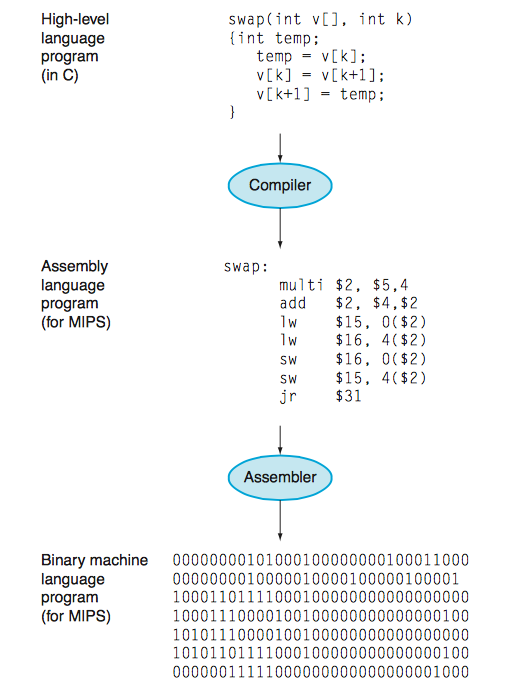
\includegraphics[height=0.9\textwidth]{img/high-level-2-low-level.png}
    \caption{Stages converting high-level language into binary machine language \protect\footnote{\cite{DAPJLH}}}
    \label{fig:hl2ll}
\end{figure}



%\section{Citations}
%Example of a citation: \cite{GRM97}, cf.\ this entry in the \Bibtex\ file.
%Another way of citing is \citep{KeR88}

%\section{Optional}
%You may wish to use the \conexp{Concept-Explorer} tool.

%\chapter{The problem and its challenges}


After presenting in the previous chapter the essential definitions for the intended work, in this chapter the project planned for this master thesis will be explained.

%Firstly, there is the necessity of generating the GIC from LISS language, like that we will see if there is no problem with the rules and definitions of a well grammar and follow the same grammar as LISS language (not being distinct) using ANTLR tool.

First, create an ANTLR version of the CFG grammar for LISS language.


Second, extend the LISS CFG to an AG in order to specify throw it the generation of MIPS assembly code.
To verify the correctness of the assembly code generated, a simple MIPS simulator, named MARS, will be selected to provide all the tools for checking it.

Third, the desired Structure-Editor, SDE, will be developed based on ANTLR.
It will be implemented in with Java SWING because ANTLR has always been implemented via Java and it is said, also, to use Java target as a reference implementation mirrored by other targets.
SWING is a GUI widget toolkit for Java which provides all the API for creating an interface with Java.
At this phase, we will create an IDE similar to other platforms but with the capacity of being a syntax-directed editor.

Fourthly, to complete the SDE functionality, an incremental compiler shall be included.
Incremental compilation ~\citep{RTD83a,Hol87a,VSK90a} means that only the part that was changed must be processed again. And like that, both tasks (edition and compilation) are done synchronously at the same time and having an editor which compiles cleverly.

Finally, exhaustive and relevant tests will be made with the tool created and, the outcomes will be analyzed and discussed.

%\section*{LISS language}


%\section{Assembly code MIPS}

%que se deve falar ?

%         The problem and its challenges.

%\section{Images}
%       Example of inserting an image as displyed text,
%\begin{center}
%       
\includegraphics[width=0.2\textwidth]{img/mei-logo-03.jpg}
%\end{center}

%\begin{wrapfigure}{r}{0.25\textwidth}
%       
\includegraphics[width=0.2\textwidth]{img/mei-logo-03.jpg}
%\end{wrapfigure}
%\noindent --- wrapped into the text,
%bla-bla bla-bla bla-bla bla-bla bla-bla bla-bla bla-bla bla-bla bla-bla bla-bla
%bla-bla bla-bla bla-bla bla-bla bla-bla bla-bla bla-bla bla-bla bla-bla bla-bla
%bla-bla bla-bla bla-bla bla-bla bla-bla bla-bla bla-bla bla-bla bla-bla bla-bla
%bla-bla bla-bla bla-bla bla-bla bla-bla bla-bla bla-bla bla-bla bla-bla bla-bla
%bla-bla bla-bla bla-bla bla-bla bla-bla bla-bla bla-bla bla-bla bla-bla bla-bla bla-bla bla-bla bla-bla bla-bla
%bla-bla bla-bla bla-bla bla-bla bla-bla bla-bla bla-bla bla-bla bla-bla bla-bla bla-bla bla-bla bla-bla bla-bla

%\noindent --- or as a floating body.
%\begin{figure}
%\begin{center}
%       
\includegraphics[width=0.5\textwidth]{img/mei-logo-03.jpg}
%\end{center}
%\caption{caption}
%\end{figure}

%You can also use an image as an icon, eg.\ \MEI, in the main tex.
%Click on it to visit the website. It is also listed in the list of terms.
%Another example of an item to appear in the term index: \UM (needs \Makeindex)


%\part{Core of the dissertation}

%\part{Core of the dissertation}

\chapter{Compiler development}
%       Main result(s) and their scientific evidence
%\section{Introduction}
Earlier in the history of computers, software was primarily written in assembly language. Due to the low productivity of programming assembly code, researchers invented a way that add some more productivity and flexibility for programmers; they created the compiler allowing to wire programs in high level programming languages.

A compiler is a software program which converts a high-level programming language (source code) into a lower level programing language for the target machine (known as machine code or assembly language).

The compiler task is divided into several steps (see Figure \ref{fig:compiler}):
\begin{enumerate}
  \item Lexical analysis
  \item Syntactic analysis or parsing
  \item Semantic analysis
  \item Optimization
  \item Code generation
\end{enumerate}

\begin{figure}
\begin{center}
       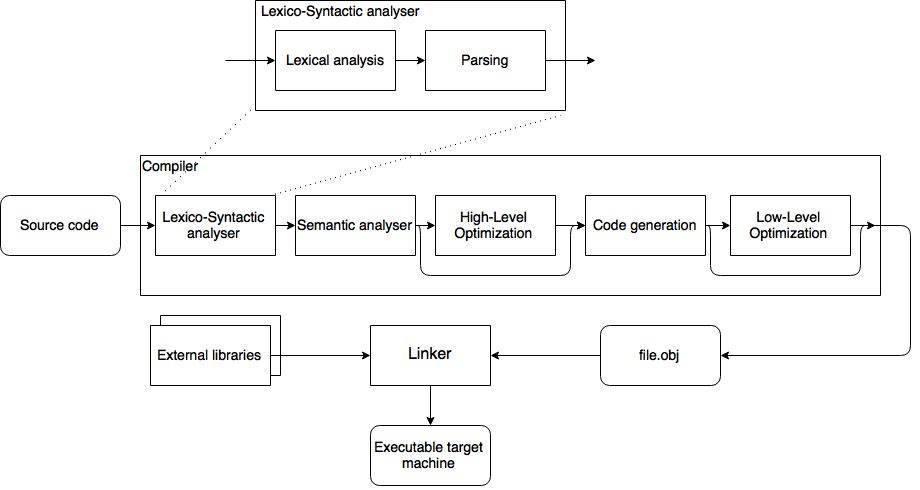
\includegraphics[width=1\textwidth]{img/compiler.png}
\end{center}
\caption{Traditional compiler}
\label{fig:compiler}
\end{figure}
\newpage
The task of constructing a compiler for a particular source language is complex. Firstly, the lexical analysis must recognize words; these words are a string of symbols each of which is a letter, a digit or a special character.

The Lexical analysis divides program text into "words" or "tokens" and once words are identified, the next step is to understand sentence structure (role of the parser).
We can think the parsing as an analogy of our world by constructing phrases which requires a subject, verb and object. So, basically, the parser do a diagramming of sentences (see Figure \ref{fig:parsing}).
\begin{figure}
\begin{center}
       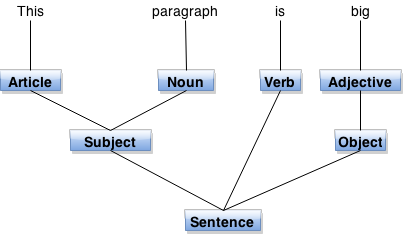
\includegraphics[width=0.7\textwidth]{img/parsing.png}
\end{center}
\caption{Parsing}
\label{fig:parsing}
\end{figure}
%\newpage
Once the sentence structure is understood, we must extract the "meaning" with the semantic analyzer.
The duty of the semantic analyzer is to perform some semantic analysis to catch some inconsistencies.
Finally, after that, it may or may not have some optimization regarding the source code. Then the code generator translates the intermediate representation of the high-level programming into assembly code (lower level programming).
\newpage
%%%%%%%%%%%%%%%%%%%%%%%%%%%

%\section{Summary}
%\section{ANTLR}
\section{Compiler generation with ANTLR}

Terence Parr, the man who is behind ANTLR (ANother Tool for Language Recognition ~\citep{parr2007,Par05}) made a parser (or more precisely, a compiler) generator that reads a context free grammar, a translation grammar, or an attribute grammar and produces automatically a processor (based on a LL(k) recursive-descent parser) for the language defined by the input grammar.

An ANTLR specification is composed by two parts : the one with all the grammar rules and the other one with lexer grammar.

Listing ~\ref{lst:agANTLR} is the one with the grammar rules; in that case it is an  example of an AG.

\begin{comment}
\begin{figure}[h!]
  \centering
    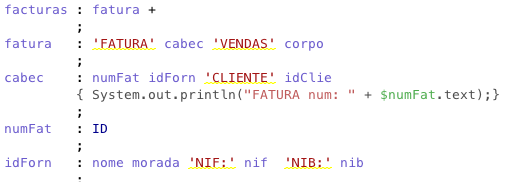
\includegraphics[width=0.8\textwidth]{img/gaAnTLR.png}
    \caption{GA representation on ANTLR}
    \label{fig:gaAntlr}
\end{figure}
\end{comment}

\begin{lstlisting}[caption={AG representation on ANTLR},label={lst:agANTLR}]
facturas : fatura +
         ;
fatura   : 'FATURA' cabec 'VENDAS' corpo
         ;
cabec    : numFat idForn 'CLIENTE' idClie
         { System.out.println("FATURA num: " + $numFat.text);}
         ;
numFat   : ID
         ;
idForn   : nome morada 'NIF:' nif  'NIB:' nib
\end{lstlisting}


On the other hand, the lexer grammar defines the lexical rules which are regular expressions as can be seen in Listing ~\ref{lst:lexer}. They define the set of possible character sequences that are used to form individual tokens. A lexer recognizes strings and for each string found, it produces the respective tokens. %(see figure~\ref{lst:lexer}).

\begin{comment}
\begin{figure}[h!]
  \centering
    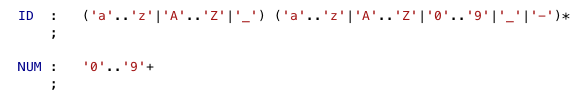
\includegraphics[width=0.8\textwidth]{img/lexer.png}
    \caption{Lexer representation}
    \label{fig:lexer}
\end{figure}
\end{comment}

\begin{lstlisting}[caption={Lexer representation},label={lst:lexer}]
/*--------------- Lexer ---------------------------------------*/

ID  :   ('a'..'z'|'A'..'Z'|'_') ('a'..'z'|'A'..'Z'|'0'..'9'|'_'|'-')*
    ;

NUM :   '0'..'9'+
\end{lstlisting}



%\newpage
The parser generator by ANTLR will be able to create an abstract syntax tree (AST) which is a tree representation of the abstract syntactic structure of source code written in a programming language (see Figure~\ref{fig:AST}).

\begin{figure}[h!]
  \centering
    
\includegraphics[width=1\textwidth]{img/antlr4_parse_tree.png}
    \caption{AST representation}
    \label{fig:AST}
\end{figure}

ANTLR will be used to generate MIPS assembly code according to the semantic rule specified in the AG for LISS language.

%The lexical syntax is usually a regular language, with the grammar rules consisting of regular expressions; they define the set of possible character sequences that are used to form individual tokens or lexemes. A lexer recognizes strings, and for each kind of string found the lexical program takes an action, most simply producing a token.


%\chapter{Applications}
%        Application of main result (examples and case studies)
%\section{Introduction}
%\section{Summary}


%%%%%%%%%%%%%%%%%%%%%%%%%%%%%%%%%%%%%%%%%%%%%%%%%%%%%%%%%%

\chapter{SDE: DEVELOPMENT}

Before we try to explain the concept of a Syntax-Directed Editor (SDE) ~\citep{RT89b,Ko05,alsCH10a,TR81a,RMT86a,RT89a,AHW89}, let's start defining what is an Integrated Development Environment (IDE).

An IDE is described as a software application that provides facilities to computer programmers for software development. It consists , normally, of a source code editor, a compiler, a debugger, and others tools.
IDEs are designed for maximizing the productivity of programmers with visual interface and contains, normally, an interpreter, a compiler or both (see Figure~\ref{fig:ideXCode}).
%IDEs are designed for maximizing the productivity of programmers with visual interface and contains, normally, an interpreter, a compiler or both (see Figure~\ref{fig:ideXCode}).


\begin{figure}[h!]
  \centering
    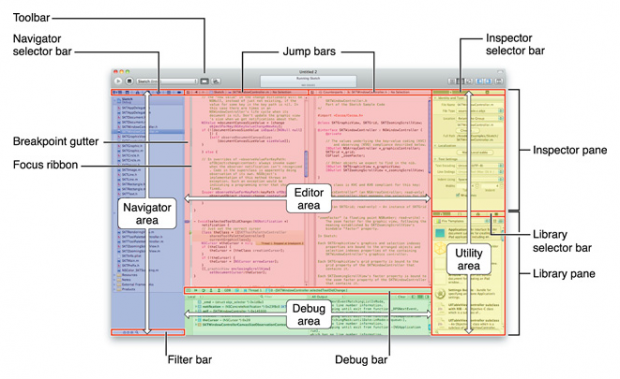
\includegraphics[width=1\textwidth]{img/XCode-interface.png}
    \caption{Example of an IDE visual interface (XCode) \protect\footnote{http://www.alauda.ro/wp-content/uploads/2011/04/XCode-interface-e1302035068112.png}}
    \label{fig:ideXCode}
\end{figure}

\newpage

Programs are created top down in the editor sections by inserting statements and expressions at the right cursor position of the current syntactic template and we can, by the cursor, change simply from one line of text to another one.

A SDE has the same approach of an IDE which is (as said above) an interactive programming environment with integrated facilities to create, edit, execute and debugging programs.
The difference between them is that SDE encourages the program writing at a high level of abstraction, and promotes the programming based on a step by step refinement process.

It liberates the user from knowing the language syntactic details while editing programs.

SDE is basically guided by the syntactic structure of a programming language in both editing and execution. It is a hybrid system between a tree editor and a text editor.

The notion of cursor is really important in the context of SDE because, when the editing mode is on, the cursor is always located in a placeholder of a correct template (see next section) and the programmer may only change to another correct template at that placeholder or to its constituents.%, and not simply from one line of text to another as an IDE alike .
%And the only place where the cursor can move anywhere is in a phrase, which can only be placed at the leftmost symbol of a template or a placeholder.

It reinforces the idea that the program is a hierarchical composition of syntactic objects, rather than a sequence of characters.

\section {What is a template?}

The grammar of a programming language is a collection of production (or derivation rules) that state how a non-terminal symbol (LHS) is decomposed in a sequence of other symbols (RHS). A template is just the RHS of a grammar rule.
Templates cannot be altered, they have placeholders for inserting a phrase or another template and they are generated by editor commands, according to the grammar production. %verificar se pode ou nao inserir placeholders


%meter example of templates !
\begin{lstlisting}[caption={Example of a IF Conditional template},label={lst:template}]
IF( condition )
  THEN statement
  ELSE statement
\end{lstlisting}

In Listing ~\ref{lst:template} we can see the editor template for the if-statement, where \textit{condition} and \textit{statement} are placeholders.

The notion of template is very important because templates are always syntactically correct for two reasons:

\begin{enumerate}
  \item First, the command is validated to guarantee that it inserts a template permitted. %at the current cursor.

  \item Second, the template is not typed, so it contains no lexical errors.

\end{enumerate}

So a correct program (i.e., a valid sentence of the programming language) is created by choosing templates and replacing placeholders by others templates or by concrets values (numeric or string constants or identifiers).

%For a better vision of the context of a SDE, see the figure ~\ref{fig:SDE}.

To clarify the definition of SDE, we will explain it with the help of an example.

\begin{figure}[h!]
  \centering
    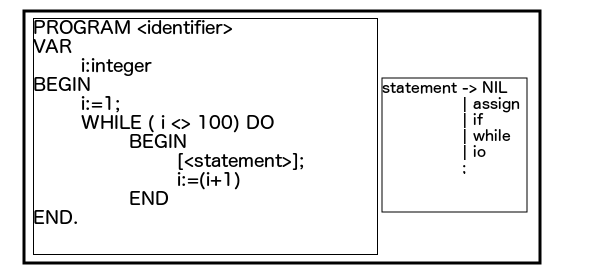
\includegraphics[width=1\textwidth]{img/SDE.png}
    \caption{SDE example}
    \label{fig:SDE}
\end{figure}

%\newpage

Figure ~\ref{fig:SDE} shows the main window of a standard Syntax-Directed Editor.
In this figure, two boxes are displayed.
The left one is the editor window where we code the program, and the right one exhibits templates choices.

Every \texttt{<}...\texttt{>}  tag represents a placeholder, and [...] represents the actual cursor position.

As the cursor changes its position, moving from one placeholder to another placeholder, the right box will be updated according to the grammar rules in the context of the new cursor position.
In this example, the cursor in Figure ~\ref{fig:SDE} is placed at the placeholder corresponding to a \textit{statement}; at the same time, the right box will be updated with all the possibile templates according to the \textit{statement} derivation rules (RHS).

To sum up, this is how a SDE works.

\section{Conception of the SDE}

%%%%%%%%%%%%%%%%%%%%%%%%%%%%%%%%%%%%%%%%%%%%%%%%%%%%%%%%%%

\chapter{Conclusion}
        %Conclusions and future work.
\section{Future Work}
%\section{Conclusion}
%\section{Prospect for future work}

	\bookmarksetup{startatroot} % Ends last part.
	\addtocontents{toc}{\bigskip} % Making the table of contents look good.
	%\cleardoublepage

	%- Bibliography (needs bibtex) -%
	\bibliography{dissertation}

	% Index of terms (needs  makeindex) -------------
	%\printindex
	
	
	% APPENDIX --------------------------------------
	\umappendix{Appendix}
	
	% Add appendix chapters
	\chapter{Liss Context Free Grammar}

	LISS ~\citep{CH07a} is an imperative programming language, defined by the Language Processing members (Pedro Henriques and Leonor Barroca) at UM for teaching purposes.
	It allows handling integers, sets of integers, dynamic sequences, complex numbers, polynomials, etc., etc~\citep{CH07d,CH07a,CH06a,CH06b,CH05a}.

	The idea behind the design of LISS language was to create a simplified version of the more usual imperative languages although combining functionalities from various languages.

	%explicar que é uma GIC de liss escrita em notaçao antlr.	
	
	\lstinputlisting[label={lst:GIC_LISS}]{lissGIC.g4}

	%\chapter{Support material}
	Auxiliary results which are not main-stream; or

	%\chapter{Details of results}
	Details of results whose length would compromise readability of main text; or

	%\chapter{Listings}
	Specifications and Code Listings: should this be the case; or

	%\chapter{Tooling}
	Tooling: Should this be the case.

	%Anyone using \Latex\ should consider having a look at \TUG,
	%the \tug{\TeX\ Users Group}


	% Back Cover -------------------------------------------
	\umbackcover{
	NB: place here information about funding, FCT project, etc in which the work is framed. Leave empty otherwise.
	}


\end{document}
